\documentclass[12pt, titlepage]{article} 

\usepackage[utf8x]{inputenc}
\usepackage{graphicx}
\usepackage{amsfonts}
\usepackage{amsmath}
\usepackage{cite}
\usepackage{colonequals}
\usepackage[hyphens]{url}


% double figures
\usepackage{caption}
\usepackage{subcaption}

\usepackage{dirtree}

% Multi-row columns in a table
\usepackage{multirow}

% Tables longer than a page
\usepackage{longtable}

% derivations
\usepackage{semantic}

% code
\usepackage{listings}
\usepackage{color}

% code definitions
\definecolor{dkgreen}{rgb}{0,0.6,0}
\definecolor{gray}{rgb}{0.5,0.5,0.5}
\definecolor{mauve}{rgb}{0.58,0,0.82}
\lstset{frame=tb,
  language=Python,
  aboveskip=3mm,
  belowskip=3mm,
  showstringspaces=false,
  columns=flexible,
  basicstyle={\small\ttfamily},
  numbers=left,
  numberstyle=\tiny\color{gray},
  keywordstyle=\color{blue},
  commentstyle=\color{dkgreen},
  stringstyle=\color{mauve},
  breaklines=true,
  breakatwhitespace=true
  tabsize=2
}

\title{Pratical Types for Python \\ Final Report}
\author{Daniel Randall \\ Imperial College London}
\date{}

\begin{document}

\maketitle


% Abstract
\begin{abstract}
Programmers spend a large percentage of their time debugging dysfunctional code. In dynamically typed languages this problem is exacerbated due to the lack of protection offered by a static compiler. Tools have been developed to ease this process but they often frustrate the user with false positives or require modification to source code. We design an out-of-the-box static type checker for a subset of the Python programming language which returns few false positives and takes an optimistic approach to Python's dynamism. We achieve this by accepting the modifications made to global variables are unpredictable and distinguishing between global and local variables in our algorithm. We take inspiration from a technique called success typings and infer the types of function arguments through the context they are used in the function body in order to prevent reliance on potentially incorrect types provided as arguments in function calls. We handle Python exceptions, which most type inferencers ignore, by assuming that all statements within a \texttt{try} are potentially exceptional. Finally we show that the subset of Python our tool covers is useful for real-world projects and how our work can be extended to cover the majority of Python functionality.
\end{abstract}

% Acknowledgements
\renewcommand{\abstractname}{Acknowledgements}
\begin{abstract}
I would like to thank my supervisors, Jeroen Ketema and Alastair Donaldson, for our many meetings and for their helpful comments.
\end{abstract}

\tableofcontents
\newpage

\section{Introduction}
\subsection{Motivation}
High level, dynamically typed languages such as Python have been gaining popularity in recent years. Python is now used as a teaching language in 80\% of the top ten Computer Science department in the USA, surpassing previous favourites such as Java~\cite{guoTeaching}. Python has also become a force in industry and has been picked up by influential software engineering companies such as Google and Yahoo!~\cite{organisationsPython}. One reason for this is a high level of productivity involved in using such languages, partly due to the programmer being free from having to declare the types of the variables used. However, the benefits gained from this design decision are at the expense of the security provided by a statically typed language. Type errors which are easily caught by a compiler for a statically typed language, such as Java or C++, can be left unnoticed in Python source code into the release stage of a product where its execution may prove fatal. \\ % Specifying types is regarded as superfluous by many in the Python community.
\indent While there has been significant talk of adding optional static typing to Python~\cite{guido1, guido2, guido3, guidoLatest}, it seems that this will be limited to annotations similar to those currently employed in the open source project mypy~\cite{mypy}. This means that even if support is added in the near future it will be some time before this is incorporated into large projects. \\
\indent Tools attempting to provide the benefits of a statically typed language to unedited Python source code do exist, such as the popular Pylint~\cite{pylint} and PyChecker~\cite{pychecker}, however their type checking ability is limited. More thorough type checker have been designed, such as Pyty~\cite{pyty} and Pyntch~\cite{pyntch}, however their usability is hampered by the the amount of configuration needed and the number of false positives returned, respectively. \\
\indent This project aims to design and implement a type checker for Python which returns few false positives. The basis for our implementation is a method called success typings~\cite{lindhal06}. We harness this idea in order to provide a over-approximation of how a function is intended to be used without relying on how the function is actually used. This allows us to determine that a violation of a function's contract is guaranteed to be a programming error. \\
\indent We introduce the general theory behind type systems in the rest of this chapter. In Chapter~\ref{chap:background} we discuss useful techniques to extract information from source code. We describe success typing as well as other type inferencing algorithms in Chapter~\ref{chap:typeinferencering}. We then examine similar tools and techniques and show the limitations in their application. \\
\indent Using the methods and techniques we described, we begin to define our solution and determine the best way to infer a type for each programming construct in Python. \\
\indent In Chapter~\ref{chap:evaluation} we evaluate our implementation. We evaluate it in four ways: the number of false positives it reports, accuracy, speed, and its ability to find bugs. We benchmark our solution against an existing type checker for Python.

\subsection{Objectives}
The objectives for this project are as follows:
\begin{itemize}
	\item \textbf{A low number of false positives} - Our solution should report a minimal number of errors which are then found not to be genuine bugs in the program. A `genuine' bug can be defined as one which is guaranteed to cause an un-caught run-time exception when executed.
	\item \textbf{Static} - Our solution should not require the user to run the program.
	\item \textbf{Out-of-the-box} - The user should not have to modify their program in any way in order to successfully use our solution.
	\item \textbf{Fast} - Our system will ideally run at a high speed, similar to other type checkers for Python.
\end{itemize} 

\subsection{Types in Programming Languages}
Type systems are created by the developers of programming languages to prevent improper use of program operations. To quote Benjamin Pierce~\cite{pierce02}:
\begin{quote}
	\emph{``A type system is a tractable syntactic method for proving the absence of certain program behaviors by classifying phrases according to the kinds of values they compute.''}
\end{quote}
In order for this to hold in programming languages, the phrases (e.g.\ variables, expressions, method calls) are labelled to express the classification. This labelling can be achieved in a number of ways and allows the language to prevent operations from being used with terms with a classification that they were not designed to be used with. \\
\indent A type system can used for detecting errors, documentation, language safety, abstraction and efficiency~\cite{pierce02}. This report focuses on error detection.

\subsection{Static and Dynamic Type Systems}
Static type systems require programs to be written such that all variables are labelled with a type. Static type systems are conservative, meaning that they can reject programs which may never cause an error at run-time. Consider the following example for the statically typed C++ language:
\begin{lstlisting}
	if (true) {	
	  int x = 5;
	} else {
	  int x = 5 + "Hello world";
	}
\end{lstlisting}
The C++ compiler will not accept this code despite the fact that it will, intuitively, behave well at run-time. This is because the type system is able to determine the \textit{absence} of type errors, that is it can determine whether code can possibly raise a type error. However, it can not detect the \textit{presence} of type errors, that is whether code which could raise a type error will ever be executed at all or in such a way that it will ever raise a type error. \\
\indent Dynamic type systems do not require types for variables until run-time where ``run-time type tags are used to distinguish different kinds of structures in the heap.''~\cite{pierce02} Dynamic type systems do not suffer from the same conservative nature as statically typed languages. For instance, the equivalent program to the previous C++ example in Python is:
\begin{lstlisting}
	if (True):	
	  x = 5;
	else:
	  x = 5 + "Hello world"
\end{lstlisting}
This program will never raise a type error, despite the fact \texttt{5 + "Hello  world"} is an illegal operation. Using a dynamic type system, only programs about to go wrong during run-time are rejected. The obvious downside to this is that errors which would be caught easily by a static type system may go undetected by a dynamic type system and wreak havoc later in the production cycle. As a trivial example of this, consider the following snippet of Python code which is a small part of a fictional large program. This program allows a user to `heal' their `characters' using `potions'. The designer has decided that the health of a character should be within a wrapper class, \texttt{Character}, and a function \texttt{add\_health} is used to combine health points:
\begin{lstlisting}
    class Character():
    # Wrapper class for the health of a character.
      def __init__(self):
        self.hp = 100
        
    class Potion():
    # Base class for potions
       def __init__(self):
         self.health_gain = 10
    
    class SpecialPotion(Potion):
    # Potion which heals a random amount
      def calculate_health_gain():
        self.health_gain = randint(0, 100)

    def add_health(character, healer):
      character.hp += healer.get_health_gain()

    def heal(character, potion):
      if potion == normal_potion:
        add_health(character, potion)
        return
      if potion == special_potion:
        calculate_health_gain(potion)
        character.hp += potion		
        return
\end{lstlisting}
Line 21 shows a legal and non-exceptional use of the code. A regular potion is used as an argument to the function \texttt{add\_health}. However on line 25 the programmer neglected to invoke the \texttt{add\_health} function for the `special potion'. The types of \texttt{character.hp} on left hand side of the assignment, type \texttt{int}, and \texttt{potion} on the right hand side, type \texttt{Potion}, are incompatible with each other and the \texttt{+=} operator and an un-caught type error will be raised if this branch is executed and the program will crash. If the programmer also neglects to include this special potion in their test suite then this code may be shipped without this branch ever having been executed. \\
\indent We can see that while dynamic type systems provide freedom, it is far easier for a type error to escape the attention of the programmer.

\subsection{Type Inference}
Type inference is the process of determining the types assigned to identifiers using the context in which they or used or the values they are assigned. When we are inferring types we assign each identifier a type. This type is a set consisting of the possible types that we believe that identifier can have at a given time. For instance, if we believe that the identifier \texttt{x} can be an \texttt{int} or a \texttt{float} at a given time then we express this by giving it the type: \texttt{\{int, float\}}.


\newpage
\section{Background}
\label{chap:background}
In this chapter we will discuss some background necessary to understand the remainder of this report. We will look at Abstract Syntax Trees which will provide a base from which we can build our algorithms. From there we will look at ways to extract information from the AST and reduce it into to a form which is easier to reason about with control flow graphs and single static assignment.

\subsection{Abstract Syntax Tree}
An abstract syntax tree (AST) ``represents the hierarchical syntactic structure of the source 
program''~\cite{dragonBook} in a tree data structure where ``each 
interior node represents an operator; the children of the node represent the 
operands of the operator.''~\cite{dragonBook} \\
\indent An AST provides us with the basis on which we can build algorithms to reason about source code. Instead of having to parse a single large string to find what what we need we can search through and manipulate the tree data structure. \\
\indent Python provides the built-in \texttt{ast} module which generates an AST from Python source code. The \texttt{ast} module transforms the following module:
\begin{lstlisting}
    x = 4
    if x == 4:
      x = 5.0 + 1
    else:
      x = "Hi"
      print(x)
\end{lstlisting}
into the following AST:
\begin{verbatim}
Module(body=[
    Assign(targets=[Name(id='x',ctx=Store())],
           value=Num(n=4))
    If(
      test=Compare(left=Name(id='x',ctx=Load()),
                   ops=[Eq()],comparators=[Num(n=4)])
      body=[Assign(targets=[Name(id='x',ctx=Store())],
                   value=BinOp(left=Num(n=5.0),op=Add(),
                               right=Num(n=1)))]
      orelse=[Assign(targets=[Name(id='x',ctx=Store())],
                     value=Str(s='Hi'))])
              Expr(value=Call(func=Name(id='print',ctx=Load()),
                        args=[Name(id='x',ctx=Load())]))])
\end{verbatim}
Each significant programming construct in Python, such as assignments, function calls and \texttt{if}s, have a corresponding class in the \texttt{ast} module. These classes have designated fields for data related to the particular construct. In the example above we can see that the \texttt{If} has three fields. One is \texttt{test} which contains a \texttt{Compare} class instance which itself contains all of the information related to the \texttt{x == 4} comparison such as the left-hand side of the comparison, \texttt{x}, the right-hand side, \texttt{4} and the type of comparison, \texttt{Eq}. The other two fields in the \texttt{If}, \texttt{body}, and \texttt{orelse} are lists with each element being a single statement within the \texttt{then} or \texttt{else} branch, respectively. \\
\indent To our knowledge, no other library which generates ASTs from Python source code, besides \texttt{ast} exists.

\subsection{Control Flow}
The control flow of an application is the route taken when the program is executed or the order in which individual statements are executed. Consider the following program:
\begin{lstlisting}
	1. x = 5
	2. x = x + 1
	3. print(x)
\end{lstlisting}
The route taken by this program is simply $1 \rightarrow 2 \rightarrow 3$. However with the introduction of conditional statements such as \texttt{if}, \texttt{for} and \texttt{while} the path taken in the program is dynamically decided by the evaluation of a condition. While the introduction of these statements undoubtedly provide more power to an engineer it is, in general, impossible to statically predict the route taken. An example of this is as follows:
\begin{lstlisting}[mathescape]
	1. if ($p_1$):
	2. 	x = 5
	3. else:
	4. 	x = 5.0
	5. print(x)
\end{lstlisting}
The flow of the above program can be described as $1 \rightarrow (2, 4) \rightarrow 5$ where $(x, y)$ represents a choice between $x$ and $y$.

\subsubsection{Control Flow Graph}
\label{chap:cfgs}
A control flow graph (CFG) is a way of depicting the control flow of a program. A CFG provides a graphical way of representing the control flow and provide a meaningful way of storing this information in a program. CFGs are commonly used in compilers in order to reduce program size and increase performance by eliminating dead code~\cite{dragonBook}. \\
\indent CFGs introduce the concept of a \textit{basic block} which consists of only straight line code and no branching statements such as ifs and loops. ``The nodes of the flow 
graph are the basic blocks. There is an edge from block B to block C if and 
only if it is possible for the first instruction in block C to immediately follow 
the last instruction in block B.''~\cite{dragonBook} Control flow statements introduce new basic blocks for each branch created by them. For example, an \texttt{if} statement creates two basic blocks, one for the then body and one for the else body. The basic blocks are then linked using directed edges with each block pointing towards its successors. \\
\indent Using the example of the \texttt{if} statement from the previous section we get:
\begin{figure}[h]
\centering
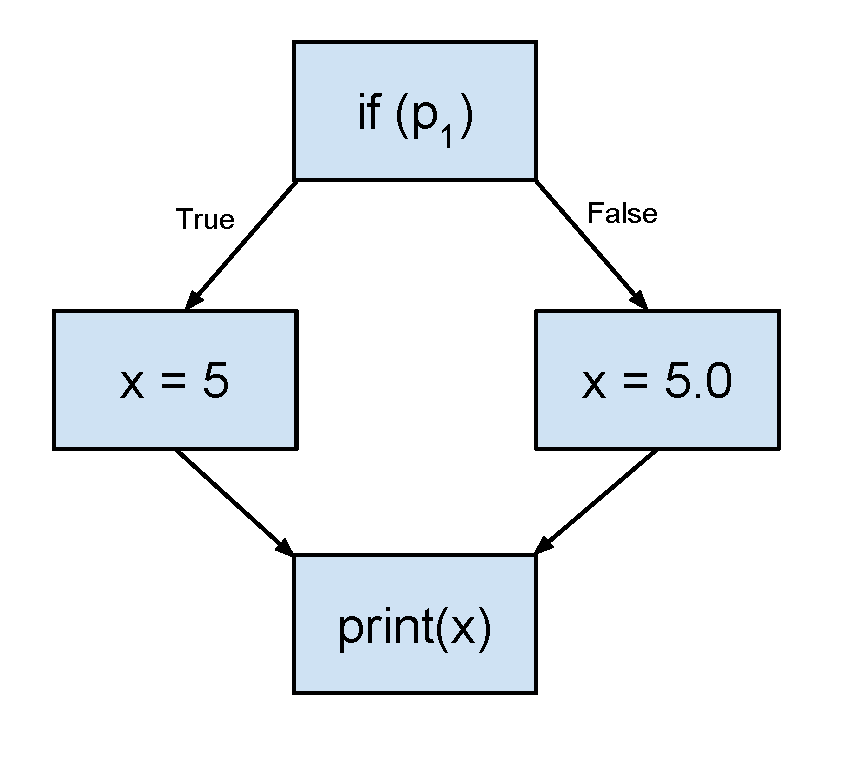
\includegraphics[scale=0.4]{images/controlFlowGraph.pdf}
\end{figure}  \\
Since the primary use for CFGs in computing is in compilers, it is natural that a good place to find a CFG generator for Python source code is in a Python compiler. The most commonly used interpreter for Python code is \textit{CPython}. CPython is written in C and uses CFGs~\cite{cpythonCFG}. CPython does not directly construct a CFG for Python code, but first transforms the code into much simpler bytecode from which a CFG is then extracted. Consider, for example, the following function:
\begin{lstlisting}[mathescape]
    def f():
      return [x for x in range(10)]
\end{lstlisting} 
CPython generates the following bytecode for this function:~\cite{cpythonBytecode}
\begin{verbatim}
    0  BUILD_LIST                     0
    3  DUP_TOP
    4  STORE_FAST                     0 (_[1])
    7  LOAD_GLOBAL                    0 (xrange)
    10 LOAD_CONST                     1 (10)
    13 CALL_FUNCTION                  1
    16 GET_ITER
    17 FOR_ITER                       13 (to 33)
    20 STORE_FAST                     1 (x)
    23 LOAD_FAST                      0 (_[1])
    26 LOAD_FAST                      1 (x)
    29 LIST_APPEND
    30 JUMP_ABSOLUTE                  17
    33 DELETE_FAST                    0 (_[1])
    36 RETURN_VALUE
\end{verbatim}
where \texttt{STORE\_FAST} stores the top of the stack (TOS) into a fast local register of the given name, \texttt{LOAD\_FAST} loads the given value in the fast local register of the given name onto the TOS, \texttt{DUP\_TOP} duplicates the reference on the TOS, \texttt{BUILD\_LIST} creates a list, \texttt{LOAD\_GLOBAL} pushes the value of the given global variable onto the stack, \texttt{LOAD\_CONST} pushes the value of the given constant on to the top of the stack, \texttt{CALL\_FUNCTION} calls a function and takes the given number of parameters, \texttt{LIST\_APPEND} calls \texttt{list.append} and looks at the given number of positions from the TOS for the value, \texttt{GET\_ITER} sets the TOS to an iterator, \texttt{FOR\_ITER} calls the TOS's iterator, \texttt{DELETE\_FAST} deletes for value of the given register and \texttt{JUMP\_ABSOLUTE} sets bytecode counter to the given value~\cite{disBytecode}. Since \texttt{f} is a one line function and results in a CFG with a single block, the CFG generated has been left out for brevity. \\
\indent In order to perform type inference on the body of function \texttt{f} we need to know that we are returning a list comprehension in which \texttt{x} is being assigned the types in the contents of the list being returned by the \texttt{range} function. Learning this information from the bytecode would not be trivial. For instance, the \texttt{RETURN\_VALUE} statement provides the value on the top of the stack as a return type of the function. Without implementing an imaginary stack it would not be clear what is being returned. Thus extracting information from such low-level bytecode is much more difficult than through accessing the designated fields in AST nodes. For this reason using a CFG built on bytecode presents needless complications and instead we shall use a CFG generated from an AST. \\
\indent \textit{PyPy} is an alternative interpreter for Python which also uses CFG generation in its tool-chain~\cite{pypyCFG}. Unlike CPython, PyPy is written in Python, however its design is very similar to that of CPython meaning it also depends on a bytecode generator to construct its CFGs. \\
\indent In 2013 a student named Ashwin Panchapakesan from the University of Ottawa built a tool to generate CFGs from Python source code~\cite{ashwinCFG}. To this end the program transforms an AST created from Python code into XML. The XML uses tags to indicate the type of a statement, such as if, while or an expression. Within these tags is the line number of the statement. The XML format of the program is then analysed in order to determine where each line number is able to flow to. The CFG generated is easy to extract from this program, however the only information contained in the XML are the line numbers making it difficult to work with. While we could just extract the matching lines of raw source code, we would then need to break down the Python syntax ourselves to extract the information to analyse. There is also no simple way to extract the necessary information from the AST based on the line numbers.

\subsubsection{Flow-sensitivity and Path-sensitivity}
\paragraph*{Flow-sensitivity}\mbox{} \\
A flow insensitive analysis of a program does not consider the order of execution~\cite{nielson99}. That is, each occurrence of a variable typically is represented by the same set of possible types no matter where it appears in the program. Consider the following example:
\begin{lstlisting}
    if (y):	
      x = 5     # S1
    else:
      x = 5.0   # S2
    f(x)        # S3
\end{lstlisting}
A flow-sensitive algorithm would infer the type of \texttt{x} at \texttt{S1} to be \texttt{\{int\}} and \texttt{\{float\}} at \texttt{S2}, while a flow-insensitive algorithm would infer the type of \texttt{x} to be \texttt{\{int, float\}} at \texttt{S1}, \texttt{S2} and \texttt{S3}. \\
\indent Another case in which ignoring the flow of execution can change the types inferred is represented by the following trivial block of code:
\begin{lstlisting}
    x = 5
    x = 5.0
\end{lstlisting}
A flow-insensitive algorithm would infer the type of \texttt{x}, for any future occurrences of \texttt{x}, to be in the set \texttt{\{int, float\}}. A flow-sensitive algorithm is able to recognise that the second statement `overwrites' the first. This permits a more accurate representation of the flow, allowing it to infer more accurately the type of \texttt{x} as the set \texttt{\{float\}}. \\
\indent A flow-sensitive algorithm is clearly the more accurate approach but requires a comparatively more complex algorithm than a flow-insensitive since the value of variables needs to be tracked at each assignment. \\
\indent Ryder~\cite{ryder03} suggests that the difference between a flow-sensitive and flow-insensitive approach is minimal in regards to object-oriented programs due to the size of methods being small. While Python can be, and is, used for object-oriented programming, a significant number of Python programs are written as scripts and so the benefits of a flow-sensitive algorithm cannot ruled out in our case.

\paragraph*{Path-sensitivity}\mbox{} \\
A path-sensitive analysis recognises the path taken at control flow constructs such as \texttt{if}s and \texttt{while}s often involve deterministic choices. To exploit this the links between blocks in the control flow graphs are labelled with the condition which needs to met for the transfer of control to take place. The feasibility of this condition in the context of its location in the program is analysed. If the link is deemed infeasible then the link is removed. The result of this procedure is a control flow graph which more accurately represents the program being analysed. However, this is more difficult than calculating flow-sensitivity due to the fact calculating the conditions statically is, in general, undecidable. For this reason, our analysis will not be path-sensitive.

\subsection{SSA Renaming}
Primarily used in compilers, Single Static Assignment (SSA) is used to acquire ``unique names for distinct entities.''~\cite{ssaBook} What this means is that each variable should only be assigned to once. There are number of variants of SSA, each designed for a specialised purpose, such as the Hashed SSA form~\cite{ssaBook} which intends to capture the fact that a single static use or definition (e.g.\ \texttt{*p} in C) could potentially impact multiple variables. In our case we are only to use a basic version of SSA, `vanilla' SSA, which we will now describe. \\
\indent Consider the following example:
\begin{lstlisting}
    x = 5
    y = x + 1
    x = 7
    z = x + 1
\end{lstlisting}
This code violates the SSA requirements since the variable \texttt{x} is assigned to twice. Translating this block into SSA form would give us the following:
\begin{lstlisting}
    x1 = 5
    y1 = x1 + 1
    x2 = 7
    z1 = x2 + 1
\end{lstlisting}
It can be observed that the most recent assignment of \texttt{x}  is used in all instances of \texttt{x} where \texttt{x} isn't being assigned a new value. This can be seen in the assignments to \texttt{y} and \texttt{z} where \texttt{x1} and \texttt{x2} is used respectively. \\
\indent Note that the names of, both, \texttt{y} and \texttt{z} need not be changed in this case since they are only assigned to once. However it often makes the implementation of SSA easier to do so regardless.

\subsubsection{The $\phi$ function}
In a straight line program the manner used to number new variables is quite intuitive, we simply increment the number appended to the end of the variable name. However, as we introduce branching into our programs this method alone breaks down. Consider the following program:
\begin{lstlisting}
    x = 5
    if (y):
      x = 5
    else:
      x = 6
    z = x + 1
\end{lstlisting}
The \texttt{if} statement has two branches which both assign a new value to the variable \texttt{x}. Assigning new names to these variables is required by the rules of SSA, however it is unclear which name we are to use after the \texttt{then} and \texttt{else} bodies, when \texttt{x} is used in an assignment to the variable \texttt{z}. \\
\indent To resolve this problem, \emph{$\phi$ function}s are used. A $\phi$ function is used ``to merge values from different incoming paths, at control-flow merge points.''~\cite{ssaBook} Put simply, the result of the $\phi$ function can be said to be \emph{any} of the parameters given to it. 
\begin{lstlisting}[mathescape]
    x1 = 5
    if (y):
      x2 = 5.0
    else:
      x3 = 6
    x4 = $\phi$(x2, x3)
    z = x + 1
\end{lstlisting}
Since we will only care about the possible types of each variable, the $\phi$ function can viewed as a glorified union of all possible types of all parameters. So in the above example we would have $\mathtt{type(x4) = type(\phi(x2, x3)) =}$ \\ $\mathtt{type(x2) \cup type(x3) = \{float\} \cup \{int\} = \{float, int\}}$. \\
\indent A similar, but slightly more complex case arises for loops. In this case, we must consider the types of the variables at each iteration of the loop as well as the exit. Consider the following trivial example:
\begin{lstlisting}
    x = 5
    while (y):
      x = x + 1.0
    z = x + 1
\end{lstlisting}
At the entry of the loop test, \texttt{y}, \texttt{x} can come from the statement immediately before the loop test, \texttt{x = 5}, as well as at the end of the loop body, \texttt{x = x + 1.0}. This can be seen clearly in Figure~\ref{fig:phiCFG} where there are two entries into the loop test where \texttt{x} may take a value. We need to represent the fact that the value of \texttt{x} at the loop test could be either of the values. We do this using the $\phi$ function. The resulting program in SSA form is:

\begin{figure}
\centering
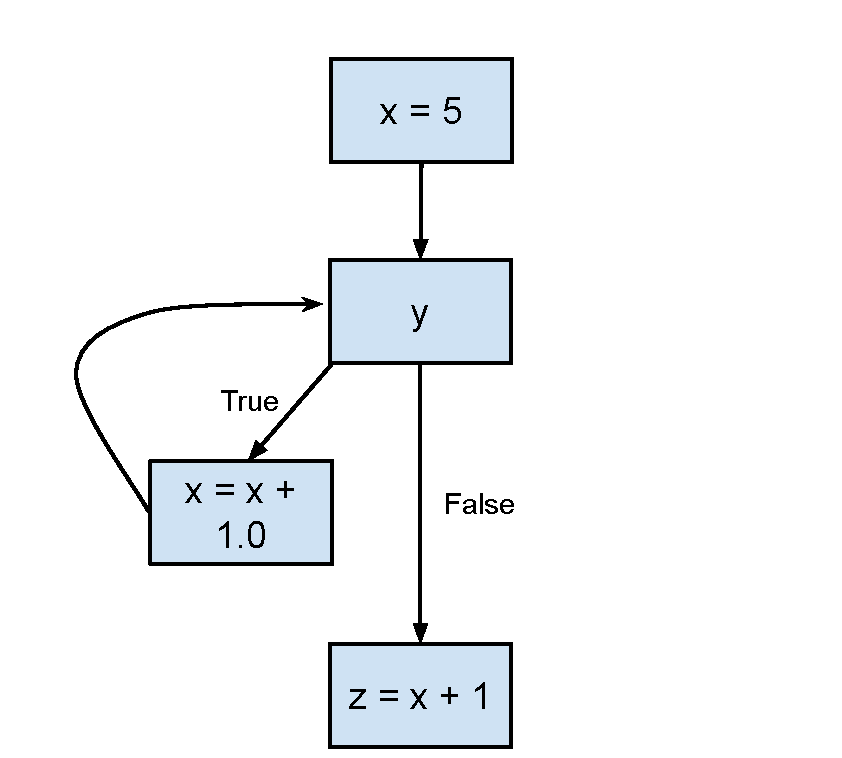
\includegraphics[scale=0.5]{images/ssaPhiNode.pdf}
\caption{A \texttt{while} loop as a CFG}
\label{fig:phiCFG}
\end{figure}

\begin{lstlisting}[mathescape]
    x1 = 5
    while (x2 = $\phi$(x1, x3), y):
      x3 = x2 + 1.0
    z = x2 + 1
\end{lstlisting}
The $\phi$ function can potentially be used for inferring the possible return types of a function. Consider the following Python function:
\begin{lstlisting}[mathescape]
    def f():
        if ($p_1$):
          return 5
        if ($p_2$):
          return "Hi"
        return 5.0
\end{lstlisting}
Here we can see that the function \texttt{f} has a number of different \texttt{return} statements which can return a number of different types. In order to infer the possible types that a function can return we need to look at the type of each return statement. We can use the $\phi$ function in order to simplify this task. To do so we modify the function as follows:
\begin{lstlisting}[mathescape]
    def f():
        if ($p_1$):
          $r_1$ = 5
          goto end
        if ($p_2$):
          $r_2$ = "Hi"
          goto end
        $r_3$ = 5.0
        end: $r_4$ = $\phi$($r_1$, $r_2$, $r_3$)
\end{lstlisting}


\paragraph*{Creating $\phi$ functions}\mbox{} \\
Since most functions do not contain a single set of variables constrained to a single control flow construct but instead have many local variables and many constructs, to create $\phi$ functions we need to know for which variables to create them. There are two ways we can go about this:
\begin{itemize}
	\item Method 1 - create a $\phi$ function for every variable within scope.
	\item Method 2 - use dominance frontiers to calculate which $\phi$ functions are necessary
\end{itemize}
Method 1 is very simple to implement. However it clearly comes with some redundancy. It will cause us to create $\phi$ functions for variables which are not modified and variables which are no longer referenced in future code. \\
\indent Method 2, dominance frontiers, eliminates redundancy at the expense of a more complicated algorithm. The algorithm is performed on code which has already been transformed into a control flow graph. The algorithm initially determines a \textit{dominance} relationship between the nodes in the CFG. Defining \textit{Entry} as the block from which function execution begins and \textit{Exit} as the block from which we return from the function, ``let X and Y be nodes in the CFG. $X$ dominates $Y$ (written $X≥Y$) if $X$ appears on every path from Entry to $Y$.''~\cite{ssaLecture} We extend this to a tighter relationship. We can say that ``$X>Y$ ($X$ strictly dominates $Y$) when $X$ dominates $Y$ but $X \neq Y$.''~\cite{ssaLecture} Using this information we can then begin to compute the dominance frontiers. ``$Y$ is in the dominance frontier of $X$ iff there exists a path from $X$ to Exit through $Y$ such that $Y$ is the first node not strictly dominated by $X$.''~\cite{ssaLecture} Having computed the dominance frontiers we add a $\phi$ function in the dominance frontier of a node for every variable assigned in that node. \\
\indent We can see an example of this process in Figure~\ref{fig:dominanceFrontiers}. We have $N>M$ and so we do not insert a $\phi$ function at $N$. However we do not have $N>Z$ and so we must insert a $\phi$ function at block $Z$. \\

\begin{figure}
	\centering
	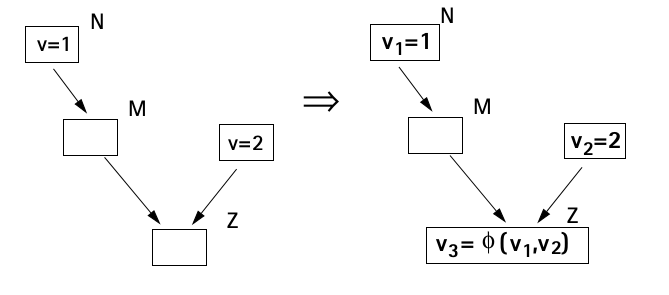
\includegraphics[scale=0.6]{images/ssaFrontiers.png}
	\caption{$\phi$ functions being placed using dominance frontiers~\cite{domianceFrontiersImage}.}
	\label{fig:dominanceFrontiers}
\end{figure} 

\indent The usefulness of SSA naming is immediately obvious. We need not track how the types of a variable may change over time. We may treat each new naming as a completely distinct variable. Managing the control flow of a program also becomes a much simpler task as we are easily able to express the fact that a variable at a given point can be a set of possible types regardless of the path taken through the program.

\subsection{Dead Code Elimination}
Dead Code Elimination is the process of detecting that a section of code is dead (unreachable) and completely eliminating it from the program. Code may be unreachable if it is placed after a \texttt{break}, \texttt{continue} or \texttt{return} statement or if the code has the effect of only modifying variables which will never be used again (`dead' variables.) The advantages of this is that we need not type check it, thus improving the speed of our program.
An example of this is:
\begin{lstlisting}
   def foo():
   	a = 24
   	b = 25     # Assignment to dead variable
   	c = a + 2
   	return c
   	b = 24 	   # Unreachable code
   	return "Hi"
\end{lstlisting}
Here, \texttt{return "Hi"} can never be reached. In addition to performance advantages, we may wish to consider removing dead code from the program in order to type functions more accurately. In the example above, if we did not eliminate dead code we will determine that the return type of the function \texttt{foo} is \texttt{\{int, string\}}. Since \texttt{int} is still part of the type, this is not incorrect but a needless overestimate. Dead code also raises some issues in how it should be handled in the CFG. Should \texttt{return c} link to \texttt{b = 24}? However, there is also an argument for type checking dead code. This code may become important later and flagging the errors may save the engineer time later on. \\
\indent Unfortunately there are no out-of-the-box solutions to this problem for Python programs. \\

\subsection{Constraints and Constraint Solvers}
Many algorithms for inferring types involve solving a set of constraints. ``A constraint satisfaction problem [CSP] is a problem where one has to find a value for a (finite) set of variables satisfying a (finite) set of constraints.''~\cite{constraintBook} A CSP is typically described using the following notation: $\langle X, D, C \rangle$. Where $X$ represents a set of variables, $D$ is a set of corresponding domains and $C$ is a set of constraints that any solution must satisfy. Every variable must have a \textit{domain}. A domain specifies the values a variable can take. An example domain is the set of integers, $\mathbb{Z}$. A solution to a CSP is a mapping from the given variables to a value in the domain which satisfies the constraints provided. \\
\indent An example of a CSP is the following, where each letter must be replaced with a different number such that the sum evaluates correctly~\cite{constraintPrinciples}: \\
\begin{equation*}
\frac{
    \begin{array}[b]{r}
      SEND \\
      + MORE
    \end{array}
  }{
    MONEY
  }
\end{equation*}
In this problem the  $\langle X, D, C \rangle$ are as follows:
\begin{verbatim}
    X:
      S, E, N, D, M, O, R, Y 
    D:
      [1..9] for S, M
      [0..9] for E, N, D, O, R, Y
    C:
      AllDifferent([S, E, N, D, M, O, R, Y])
      ExactSum([SEND, MORE], MONEY)
\end{verbatim}
where \texttt{AllDifferent} is shorthand for $S \neq E \neq N \ldots$ and similarly \texttt{ExactSum} is shorthand for $(S \times 1000 + E \times 100 \ldots)  + (M \times 1000 + O \times 100 \ldots) = (M \times 10000 + O \times 1000 \ldots) $ \\
\indent There is a single solution to this CSP:
\begin{verbatim}
    S = 9, E = 5, N = 6, D = 7, M = 1, O = 0, R = 8, Y = 2
\end{verbatim}
Constraints are frequently solved using constraint solvers. % A third-party constraint solving package for Python called \textit{python-constraint}. python-constraint provides a number of built-in constraint types to use such as \textit{NotInSetConstraint}, \textit{AllEqualConstraint} and \textit{ExactSumConstraint}. However, it also allows you use a \textit{FunctionConstraint} to which you provide a function defining the constraint logic. This means the constraints it can handle are endless.

\newpage
\section{Type Inferencing Algorithms}
\label{chap:typeinferencering}
The main problem which is required to be solved by this project is how to statically infer the types for Python programs. \\
\indent In this section we look at a number of the existing techniques to achieve this while keeping in mind the objectives described at the beginning of this report. Those were, for our tool to return a low number of false positives, for it to statically analyse the code (not run it), for it to be an out-of-the-box solution and for it to be reasonably fast.

\subsection{Hindley-Milner}
The Hindley-Milner algorithm was developed by Robin Milner based on the work of J. Roger Hindley. Hindley described the \textit{principal
type schema}~\cite{hindley69}, ``which is the most general polymorphic type of an expression, and showed that if a combinatorial term has a type, then it has a principal type.''~\cite{cardelli87} Milner's contribution was an extension to Hindley's \textit{principal type schema} which included the ``notion of generic and non-generic type variables, which is essential for handling declarations of polymorphic functions.''~\cite{cardelli87} Milner's work culminated in the type inference system for the ML language~\cite{milner84}. \\
\indent The Hindley-Milner algorithm uses the operations performed on expressions to generate constraints on the types of those expressions. This is done by annotating the nodes of an expression tree with the constraints in a bottom up fashion\footnote{The Hindley-Milner algorithm can be implemented top-down, called the $\mathcal{M}$ algorithm, or bottom-up, called the $\mathcal{W}$ algorithm~\cite{heeren02}. However, the bottom-up version appears to be much more common.}. \\ 
\indent The constraint is solved to infer a type for a term using a \textit{unification} algorithm. \\
\indent For an example of how the algorithm is performed, consider the following function written in Standard ML~\cite{cannonlocalizedtype}:
\begin{lstlisting}
    fun foo x y =
      if x = y
        then x - y
        else x + y
    ;
\end{lstlisting}
Using the $\mathcal{W}$ version of the algorithm, the function is determined to have parameter types \texttt{(\{int\}, \{int\})} and return type \texttt{\{int\}}. This is calculated in five steps. \\
\indent The first step is to initialise the function parameters to empty type variables, \texttt{a} and \texttt{b}. \\
\indent In the second step we analyse the \texttt{if} test. Standard ML requires two variables to be of the same type to be legally compared. The statement on line 2, \texttt{if x = y}, imposes the constraint on the two type variables, \texttt{a = b}, or $\mathtt{a \subseteq b}$ and $\mathtt{b \subseteq a}$. \\
\indent In the third step, the \texttt{then} branch is evaluated. Standard ML only permits the \texttt{int} type to be used in conjunction with the \texttt{-} operator. The types of \texttt{a}, and therefore \texttt{b}, is set to the \texttt{int} type. \\
\indent For the fourth step, the \texttt{else} branch is evaluated but no new constraints are imposed. The restriction created by the \texttt{+} operator is the same as that for the \texttt{-} operator. \\
\indent The final step determines the return type of the function. Since the \texttt{if} statement is the only expression in the function. Both branches result in an \texttt{int} type and so the return type of the function is determined to be type \texttt{int}. \\
\indent Bugs can be detected using Hindley-Milner by determining whether there are inconsistencies in the set of constraints.

\paragraph{Limitations}\mbox{}\\
The technique does not allow a polymorphic argument to be of a different type in different locations. This is because unification requires there to be a single type for all appearances of a variable. For this reason Hindley-Milner is unable to infer a type for programs such as the following:
\begin{lstlisting}
	if (y):	
	  x = 5     
	else:
	  x = 5.0   
\end{lstlisting}
We have already seen examples such as this in previous chapters, and so the Hindley-Milner approach is not appropriate in our case.

\subsubsection{Pyty}
Developed by Jeff Ruberg~\cite{pyty}, Pyty is a bug checker which analyses annotated source code to detect errors related to the misuse of types. Pyty employs Hindley-Milner as its type inferencing algorithm. Pyty works upon a subset of Python, TPython. Types are inferred using a defined abstract grammar and a series of typing rules. The source code is analysed using mild type inference alongside the type annotations to extract type information. This information is compared with the type rules in order to determine whether the program types correctly.
\paragraph{Limitations}\mbox{}\\
Pyty requires annotations to the source code in a specific format, such as the following: \texttt{fib : int -> int} where the function \texttt{fib} accepts an \texttt{int} as an argument and returns an \texttt{int}. This is quite tedious and prevents it from being an `out-of-the-box' solution to our problem.

\subsection{Palsberg and Schwartzbach Algorithm}
The Palsberg and Schwartzbach algorithm~\cite{Palsbergstatictyping} works by constructing a network of constraints where each expression in the analysed program is represented by a node in the network. The node contains the types which the expression may assume during execution. All types are initially set to be empty except from constants and literals. The constraints between the nodes are created in response to statements in the program. In the Palsberg and Schwartzbach algorithm there are two ways in which a constraint can generated: assignments and function calls. An assignment such as $\mathtt{x := y}$ is represented by the constraint $\mathtt{type(x) \subseteq type(y)}$. Function calls generate constraints between the \textit{actual} arguments used in the function call and the formal arguments in the function definition. The constraints are solved by propagating types through the constraint edges until a fixed-point is reached. Consider the following toy example: 
\begin{lstlisting}
    fun f(x):
      y = x
      
    f(3)
\end{lstlisting}
For this code, two constraints are generated. A subset constraint between the value \texttt{3} and the parameter \texttt{x} in \texttt{f}, $\mathtt{type(3) \subseteq type(x)}$, and between the parameter \texttt{x} and the local variable \texttt{y} in \texttt{f}, $\mathtt{type(x) \subseteq type(y)}$.  \\
\indent The algorithm is used for object-oriented code by copying the bodies of base classes inherited into the child classes. Similarly, class definitions are duplicated at all sites at which they are constructed and method bodies are duplicated at call sites.
\paragraph*{Limitations}\mbox{}\\
The excessive duplication makes the algorithm impractical. In the worst case, successive expansions squares the size of the program to be analysed.


\subsection{Cartesian Product Algorithm}
The Cartesian Product Algorithm (CPA) was originally conceived by Agesen as an improvement on the Palsberg and Schwartzbach algorithm for the language Self~\cite{agesen95}. \\
\indent The Cartesian Product Algorithm works by modelling data flow, as done in the Palsberg and Schwartzbach algorithm, as opposed to the constraint and unification method adopted by the Hindley-Milner algorithm. This is done by building a set of possible types an expression can take. Consider the following code:
\begin{lstlisting}
    if (y):	
      x = 5     
    else:
      x = 5.0  
\end{lstlisting}
The inferred type for \texttt{x} would be the set $\mathtt{\left\{ {int, float}\right\}}$, where the possible \texttt{int} type is found in the \texttt{then} branch and the \texttt{float} type is found in the \texttt{else} branch. The types from each branch are unioned to the set of possible types for \texttt{x}. The CPA algorithm guarantees that the type of the variable is contained within the set. \\
\indent In order to infer the types handed to a function the cartesian product of the set of possible types for all given arguments is taken. Consider the following code:
\begin{lstlisting}
    if (y):	
      x = 5 
      z = "Hello world"    
    else:
      x = 5.0 
      z = True
    f(x, z)
\end{lstlisting}
The set of inferred types for \texttt{x} is, as before, $\mathtt{\left\{ {int, float}\right\}}$ and the set for \texttt{z} is $\mathtt{\left\{ {string, bool}\right\}}$. The possible types of the inputs to the function \texttt{f} are: $\mathtt{\left\{ {int, float}\right\} \times \left\{ {string, bool}\right\} = \{ (int, string), (int, bool),(float, string),}$ \\ $\mathtt{ (float, bool)\}}$, where each tuple represents the possible types of the variables given to \texttt{f}. \\
\indent The biggest shortcoming of the Palsberg and Schwartzbach algorithm, the excessive code duplication, was reduced by the CPA algorithm. This was done by duplicating function bodies such that they contain an argument list with monomorphic types which Agesen calls templates. Each argument list generated by taking the cartesian product at calls sites is connected with constraints to the corresponding template. The types of the values returned by each template are connected to the result of the function call. While duplication still occurs, it is bound by the number of possible combinations of the types of the arguments, rather than being duplicated each time for every function call.
\paragraph*{Limitations}\mbox{}\\
The size of the Cartesian products grows exponentially with the number of arguments given to the function call. However the size is bounded by the number of types available. \\
\indent The difficulty of implementation is greater than that of the Hindley-Milner algorithm which is known as being a fairly simple algorithm to implement~\cite{jones95}. \\
\indent Taking the cartesian product of the possible types given to a function call is unnecessary if the possible types the function can take are already known. \\
\indent While duplication has been reduced in comparison to the Palsberg and Schwartzbach algorithm, each function body is still duplicated to generate all possible templates.

\subsubsection{Starkiller}
Starkiller was designed by Michael Salib as a Python-to-C++ compiler~\cite{starkiller}. The type inference algorithm used was based on Agesen’s Cartesian Product Algorithm. Starkiller generates a dataflow networks which is populated with nodes for all variables and expressions in the program and links these nodes together through a series of constraints. Concrete types are then propagated through these constraints. Starkiller achieves complete type inference for a subset of Python.
\paragraph*{Limitations}\mbox{}\\
Starkiller is unable to infer types for the dynamic constructs such as \texttt{eval}, or \texttt{exec}, nor does it support exceptions of any kind. The implementation is flow-insensitive and so all variables are typed as the union of all types it can have at each of its occurrences. This means Starkiller is not precise. Frequently used language constructs such as exceptions, iterators and generators are not supported. The types of function arguments are inferred from the call sites, however this is not a problem since Starkiller is not a bug checker and so the Python source code being analysed, and thus the arguments given to a function call, are assumed to be correct.

\subsubsection{Shed Skin}
Shed Skin is a Python-to-C++ compiler developed by Mark Dufour which boasts an up to 40-fold performance increase over an older Python-to-C++ compiler, Psyco~\cite{shedskin}. Shedskin employs the Cartesian Product Algorithm (CPA) alongside iterative class-splitting. The CPA algorithm is used to allow the user to know which functions need to be defined. For instance, if Shed Skin comes across \texttt{max(1, a)} where \texttt{a} can be the types in the set \texttt{\{int, float\}} the \texttt{max} function needs to be duplicated in C++ to cover \texttt{max(int, int)} and \texttt{max(int, float)}. Dufour also needs to define classes for the types used. For data polymorphic types such as lists, the class cannot always be shared so the the classes are `split' once they can no longer share the same representation of data in the equivalent C++ program.

\paragraph*{Limitations}\mbox{}\\
The programs consumed by Shed Skin are required to be implicitly statically typed. Meaning the type of a variable can not dynamically change. Shed Skin also does not support a number of Python features such as \texttt{eval} and \texttt{isinstance}.

\subsubsection{Localized Type Inference of Atomic Types in Python}
For his masters thesis, Brett Cannon attempted to infer the types for local, atomic (built-in) variables. This is done in an attempt to improve the performance of Python~\cite{cannonlocalizedtype}. The algorithm used by Cannon is based on a variation of the CPA algorithm. The difference being that the type inference is performed by intercepting bytecode from the interpreter. The bytecode is then modified by injecting additional bytecode relating to the types of variables. The aim is to provide type information which can be utilised to improve performance. Cannon's work differs to Psyco, a previous performance-boosting tool, in that the work is done inside Python's compiler, rather than the interpreter.
\paragraph{Limitations}\mbox{}\\
The inference is limited to built-in types: \texttt{integrals}, \texttt{float}, \texttt{complex}, \texttt{basestring}, \texttt{list}, \texttt{tuple} and \texttt{dict} so any user-defined types are ignored. \\
\indent Cannon's work is only able to infer types for local variables, meaning that the implementation is largely useless when used on programs designed with Object Oriented Programming (OOP) in mind, as noted by Cannon. While not a real limitation, Cannon's solution intercepts the compiler in order to improve performance. This is not our aim and we need not complicate things by working with bytecode.

%\subsection{Gradual Typing}


\subsection{Success Typings}
The phrase `success typings' was coined by Lindhal and Sagonas in the 2006 paper \textit{Practical Type Inference Based in Success Typings}~\cite{lindhal06}. The aim of a success typing is to fully describe all possible intended uses of a function. To do this the types of the parameters are inferred by observing the context in which they are used within the function. The description of a function is given as type signature for a function $f$: $(\bar{\alpha}) \rightarrow \beta$, where $(\bar{\alpha})$ refers to the type of the function parameters, and $\bar{\alpha}$ is a shorthand for $\alpha_1, \alpha_2,...\alpha_n$, and $\beta$ is the type of the return value. Both types are the `largest' possible types, i.e.\ subtypes are acceptable. For instance, consider the following function as described in the Lindhal et al.\ paper for the functional language \textit{Erlang}:
\begin{lstlisting}[mathescape]
	and(true, true) $\rightarrow$ true;
	and(false, _) $\rightarrow$ false;
	and(_, false) $\rightarrow$ false;
\end{lstlisting}
where the symbol `\_' represents a \textit{don't care} option for pattern matching, meaning it will match any value for the corresponding parameter. \\
\indent An acceptable success typing for this function, and, indeed, for any function with two arguments, would be: $(any(), any()) \rightarrow any()$ where $any()$ denotes the set of all Erlang types. Such a typing would raise no warnings about any use of the function and so can be used when no typing information can be inferred about a function. However, a more useful typing for the function in question is $(any(), any()) \rightarrow bool()$ where the return type of the function is restricted to all subtypes of $bool()$. Since we have the \textit{don't cares} any parameter paired with an instance of $false$, such as $(42, false)$, constitutes a valid use of the function. This optimistic approach avoids any possible false positives and so will never reject a well-formed program. This typing does allow for warnings to be issued as a result of type clashes in matching a value which is not a subtype of $bool()$ with the result of the function. \\
\indent A success typing is inferred by building constraints by traversing the code and then solving them. \\
\indent Constraints are built based on a number of derivation rules. Assume the following definitions: \\
\indent The symbol $e$ is any expression which can be defined in the language under consideration, $\tau$ is a type, such as a boolean or integer, $A$ represents an environment with bindings of variables of the form $\{\ldots, x \mapsto \tau_x, \ldots\}$, $C$ represents nested conjunctions and disjunction of subtype constraints, $V$ represents the possible type variables, $P$ represents the set of all possible concrete types, $T$ represents the set of possible types and variable may assume, $T \text{ when } C$ represents a type resulting from certain constraints being satisfied and $c(T_1, \ldots, T_n)$ are structured types, such as tuples.
\begin{align*} 
	C \coloncolonequals (T_1 \subseteq T_2) \mid (C_1 \land \ldots \land C_n) \mid (C_1 \lor \ldots \lor C_n)
\end{align*}
\begin{align*} 
	T \coloncolonequals none() \mid any() \mid V \mid c(T_1, \ldots, T_n) \mid (T_1, \ldots, T_n) \rightarrow T'\mid T_1 \cup T_2 \mid T \text{ when } C \mid P
\end{align*}
\begin{align*} 
	V \coloncolonequals \alpha, \beta, \tau
\end{align*}
\begin{align*} 
	P \coloncolonequals integer() \mid float() \mid atom() \mid pid()\text{ } | \text{ 42 } | \text{ foo } | \ldots
\end{align*}
and the judgement $A \vdash e : \tau, C$ should be read as ``given the environment $A$ the expression $e$ has type $Sol(\tau)$ whenever $Sol$ is a solution to the constraints in C.'' \\
\indent Then one such derivation rule is the rule for a struct:
                \[
\inference*[STRUCT]{  A \vdash  e_1 : \tau_1, C_1 \ldots e_n : \tau_n, C_n}
                                        {A \vdash  c(e_1, \ldots, e_n) : c(\tau_1, \ldots, \tau_n), C_1 \land \ldots \land C_n}
                \]
The rule states that given a number of elements, each with its own type, it is possible to group them into a tuple structure with each individual element retaining their type. The constraints for each element are added to the environment in a conjunction. \\
\indent $Sol$ is a mapping from type expressions and type variables to concrete types. $Sol$ is a solution to a constraint set $C$ if:
\begin{align*} 
	Sol \models T_1 \subseteq T_2 \iff none() \subset Sol(T_1) \subseteq Sol(T_2)
\end{align*}
\begin{align*} 
	Sol \models C_1 \land C_2 \iff Sol \models C_1, Sol \models  C_2
\end{align*}
\begin{align*} 
	Sol \models C_1 \lor C_2 \iff \begin{cases} Sol_1 \models C_1, Sol_2 \models C_2, \\
	                                            Sol = Sol_1 \sqcup Sol_2 \end{cases}
\end{align*}
where $Sol_1 \sqcup Sol_2$ denotes the point-wise least upper bound of the solutions. This means the least general types are taken which satisfies bought $Sol_1$ and $Sol_2$. The algorithm iterates until this is found. \\
\indent Each case represents a different type of constraint which we may encounter (subtype, conjunction or disjunction). The subtype case states that a solution satisfies a subtype constraint if the mapping satisfies the subtype constraint and neither of its constituents is \textit{none()}. The conjunction case states that the solution must satisfy all conjunctive parts. The disjunction case states that the solution is the point-wise least upper bound of all disjuncts. \\
\indent To our knowledge, success typings has not been implemented in any language other than Erlang.
\paragraph{Limitations}\mbox{} \\
The primary limitation of success typings is that it resorts to labelling a function parameter as having the type $any()$ if it is unable to infer the possible types which results in inaccuracy. Lindhal and Sagonas had success in implementing success typings for Erlang. However Erlang is a functional language and activity within the code is largely limited to functions making the number of possible ways the parameter can be used to be quite small. Their success may be more difficult to replicate in object-oriented and imperative languages, such as Python.


\subsection{Soft Typing}
Cartwright and Fagan extended the Hindley-Milner $\mathcal{W}$ algorithm to introduce soft typing~\cite{cartwright91}. The aim of soft typing is not to reject a program for which static type checking fails but to ``transform arbitrary programs to equivalent programs that type check.'' Soft typing works by inserting run-time checks, resulting from ``narrowers,'' when a program fails to statically type a program, i.e.\ when unification in $\mathcal{W}$ fails. Narrowers are type casts which blindly convert from the current type to the destination type. Conversion errors are caught by the run-time checks.
\paragraph{Limitations}\mbox{} \\
Soft typing requires a program to be executed in order to notify the programmer about errors. Our aim is to create a static debugger and so our aims are incompatible with soft typing.

\subsection{Aggressive Type Inference}
Aggressive type inference (ATI) is a technique developed by John Aycock~\cite{aggressiveType} which follows the idea that:
\begin{quote}
	\emph{``Giving people a dynamically-typed language does not mean that they write dynamically-typed programs.''}
\end{quote}
Aycock backs up this hypothesis by citing a study which reveals that around 80\% of operators in a set of \textit{Icon} programs maintain the same type throughout their lifetime~\cite{typeInferenceIcon}. \\
\indent He exploits this by using a flow-insensitive method and does not use union types. This means that the algorithm does not look through all routes to determine all possible types for a variable and only labels a variable with a single type, not a union of multiple types. The algorithm works by iteratively analysing the code to infer the types of variables and by propagating the types on each iteration.
\paragraph{Limitations}\mbox{}\\
The limitations of Aycock's approach are quite clear: the types involved in dynamic behaviour are not reliably extracted. How much of an issue this poses is up for debate;
A study on this, more recent and relevant to our interests than the \textit{Icon} analysis put forward by Aycock, has been conducted by Alex Holkner and James Harland~\cite{evaluatingDynamicBehaviour}. This study details the evaluation of twenty-four open source Python programs. They observe that dynamic features are actually widely used. For instance, they find that all systems studied employ dynamic code execution. Holkner and Harland concede that their study is small in comparison to the amount of Python code available, however if their results are to be extrapolated then Aycock's assumption is not so reasonable.

\subsection{PyPy}
RPython is an intermediate language, a subset of Python which is entirely statically typed and which acts as a link in the PyPy toolchain~\cite{pypyRpython}. PyPy's goal is to develop a Just-In-Time (JIT) compiler for Python. PyPy's interpreter is written in RPython which removes dynamic features in order to reduce the complexity of type inference.
\paragraph{Limitations}\mbox{}\\
The major limitation of PyPy is the use of RPython. One feature of RPython is that it does not allow variables to change their type.

\subsection{Related Work}
To the best of our knowledge, there is currently no bug finder for type errors in Python which does not return any false positives. The most used code analysis tools at the time of writing are Pylint and and PyChecker.
%\subsubsection{Psyco}
%Psyco is a just-in-time (JIT) compiler for Python, designed to improve performance~\cite{psyco}. Psyco replaces the main interpreter loop of Python in order to examine the bytecode and, where appropriate, emits specialized bytecode in its place. CITATION NEEDED
%\paragraph*{Limitations}\mbox{}\\
%Psyco only attempts to infer locally defined \textit{ints} and \textit{strings} and pays little interest to any other types.

\subsubsection{Pylint}
Pylint~\cite{pylint} is an error checking tool for Python which statically analyses Python source code to look for errors and to assess the coding style. Pylint is a static analyser and so it looks for errors without running the source code. \\
\indent Documentation on Pylint is almost non-existent and the source code is also quite difficult to understand so, unfortunately, we currently do not understand the type inference algorithm of Pylint.
\paragraph{Limitations}\mbox{}\\
Pylint can often return a lot of false positives and offers a large number of command-line options in an attempt to allow users to manually suppress them. However the false positives are generally not related to the type checking performed by Pylint. The reason for this is that type checking performed by Pylint is limited. For example, the types of the arguments passed to functions are not checked.

\subsubsection{PyChecker}
PyChecker~\cite{pychecker} is a bug checker for Python which checks for type errors among a host of other errors. PyChecker is similar to Pylint except it does not check the coding style of the source program. PyChecker also differs in that it needs to runs the code in order to analyse it.
\paragraph{Limitations}\mbox{}\\
The type inference is quite limited. PyChecker focuses on `softer' type errors, such as whether a variable exists and whether \texttt{self} is the first method argument. \\
\indent PyChecker can return spurious errors and warnings. PyChecker imports the code it is analysing which, due to the fact importing executes top-level code, can have undesirable side effects, such as executing a database query in the code. \\


\subsubsection{PySonar}
PySonar was developed by Yin Wang while an intern at Google between 2009 and 2010 and was intended for the internal use within Google's Grok project~\cite{pySonar}. PySonar was primarily developed as a tool to allow the user to better search and understand Python code. It includes a type inferer in order for the types of variables to be displayed in a tooltip. It also includes an indexer to allow quick search through code. PySonar uses abstract interpretation to infer the types of the variables. PySonar claims to be able to resolve the names of 97\% of the Python standard library.
\paragraph{Limitations}\mbox{}\\
PySonar is focused on indexing the code it analyses and so it does not report any possible type errors. The program focuses mainly on a less dynamic subset of Python which is `easier' to analyse.

\subsubsection{Pyntch}
Created by Yusuke Shinyama, Pyntch uses type inference in Python in order to find bugs~\cite{pyntch}. The method used is `type flow analysis', which is a form of data flow analysis where the types are tracked as they flow from variable to variable. The documentation on the algorithm used by Pyntch is limited. For this reason we do not fully understand the method used. Project activity seems to have ceased since 2009.
\paragraph{Limitations}\mbox{}\\
Pyntch completely disregards execution order. In the following example given by the author:
\begin{lstlisting}[mathescape]
    x = 1
    x = 'a'
\end{lstlisting}
The variable \textit{x} will always have the type \texttt{\{int, string\}} after analysing the second statement. \\
\indent Pyntch is unable to infer types in code which use the following functions: \texttt{globals},  \texttt{locals},  \texttt{getattr},  \texttt{setattr},  \texttt{eval},  \texttt{compile} or  \texttt{exec}. \\
\indent As well as the inaccuracies listed, the Pyntch author states that ``sometimes Pyntch brings a lot of false positives in its result, which need to be further examined by human programmers.''

%\subsection{Javascript}
%Javascript is a dynamically typed scripting language, similar to Python. \\
%Abstract interpretation lattice \\


\subsubsection{Ruby}
Ruby is a dynamically typed scripting language, similar to Python. Due to the similarities of the languages, we will look at some related work in Ruby in the hope there are transferable techniques we can employ. \\
\indent Furr et al. developed Diamondback Ruby (DRuby)~\cite{furr09} in order to discover type errors. DRuby works by using type annotations of library functions in order to generate constraints to infer the types for user defined functions. DRuby is an aggressive error checker and so reports false positives. \\
\indent An extension to Diamondback Ruby, $\mathcal{P}$Ruby, was created in order to handle difficult dynamic language constructs such as the \texttt{eval} method which converts a string into executable program code~\cite{pRuby}. This is done by instrumenting the code such that, when the program is run, all uses of the dynamic constructs are recorded. This allows a \textit{profile} to be built which fully describes how they were used. With this profile the dynamic code can be inserted into the program in place of the dynamic constructs. The modified program can then be statically analysed just like any other. Furr et al. use DRuby for the analysis. Since this process involves running the code it offers no real solution to typing \texttt{eval} in regards to static analysis.





\newpage
\section{Design of the Type Inferencing Algorithm}
\label{chap:designAlg}
Our primary aim is to create a type checker for Python which returns a minimum amount of false positives. This decision has largely dictated the design of our algorithm. We take a cautious approach to handling exceptions. We do this by assuming that every statement within a \texttt{try} is capable of causing an exception and leading to the exception handlers. \\
\indent We assume that any code written by the programmer is possibly incorrect. Due to this restriction we can not use the function calls to determine the types taken by function arguments, the technique adopted by most of the type inferencers described in our background research. For this reason we follow the ethos of success typings which is to infer types for function arguments by observing the context in which they are used in the function body. \\
\indent We treat global variables separately from local variables. We do not attempt to determine which types a global variable can have at certain points in a program, a task which is perhaps impossible. Therefore we assume global variables can be all of the possible types they can take at all times. However the path taken by local variables is easier to determine and so we perform this analysis in order to improve accuracy. Due to this it can be said we take a flow-sensitive approach for local variables and flow-insensitive approach for global variables.  \\
\indent We only issue an error if there is no type which can be legally used in a given context. This decision was made to minimise the number of false positives. Consider the following code:
\begin{lstlisting}[mathescape]
    def f():
      if some_condition:
        return 5
      else:
        return None
        
    x = f()
    y = x + 1
\end{lstlisting}
The function \texttt{f} has the return type \texttt{\{int, None\}}. In line 7, the variable \texttt{x} has been assigned the return values of \texttt{f} and so also has the type \texttt{\{int, None\}}. In line 8, \texttt{x} has been used in the binary operation \texttt{+} with the integer \texttt{1}. The only legal types which can be legally used in conjunction with the \texttt{int} type in a binary \texttt{+} operation is \texttt{int} and \texttt{float}. This means that if the function \texttt{f} returns the \texttt{None} type then there will be a type error on line 8. However we do not know that the \texttt{if} in line 2 will ever evaluate to false and cause function \texttt{f} to return \texttt{None}. If the \texttt{if} always evaluates to true then issuing  an error will constitute a false positive. For this reason we do not issue an error if there is at least one type which can be legally used in a given context.

\newpage
\section{Implementation}
All of the implementation was created using the Python language. As this allows us to use the built-in \texttt{ast} module which provided the base from which this project was built. No other language offered such a critical component out-of-the-box. \\
\indent To implement flow-sensitivity for local variables, we use single static assignment. SSA allows us to use a flow-sensitive approach while implementing a simpler flow-insensitive algorithm in our type checker. \\
\indent The basic structure of our system can be seen in Figure~\ref{fig:systemStructure}. The basic components are the AST, CFG, SSA, Preprocessing and Type Inference. Each component will be described here. \\
\indent This traverser used to navigate the AST are taken from Edward K. Ream's \textit{stc}~\footnote{\url{https://code.launchpad.net/~edreamleo/python-static-type-checking/trunk} Revision \#448 was used for this project.}.


\begin{figure}
\centering
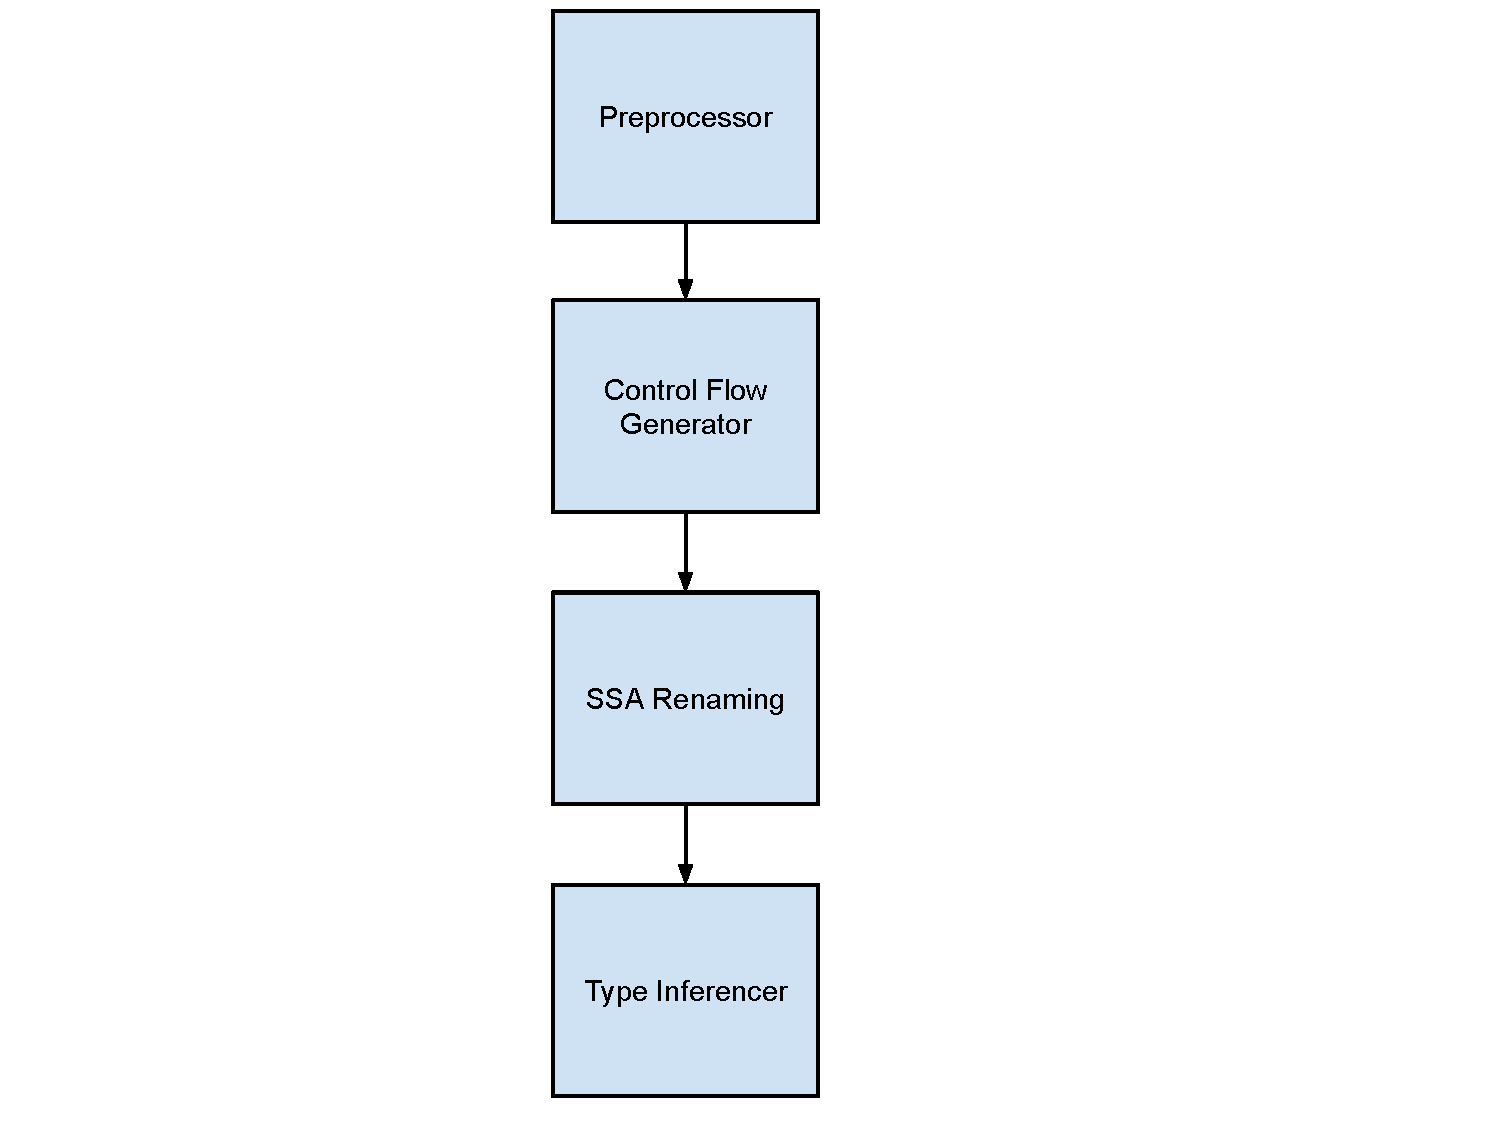
\includegraphics[scale=0.5]{images/systemStructure.pdf}
\caption{Each box represents a key component of the system. Arrows represent the flow of information from each component to another.}
\label{fig:systemStructure}
\end{figure}

\subsection{Preprocessing}
The preprocessing step is designed to modify the AST generated by the \texttt{ast} module in order to simplify the further steps. Some information extraction is also performed, the context of each node is calculated (such as whether the node is contained in a module, function or class,) as is the list of global variables in modules and classes. \\
\indent We will discuss how we manipulate some tricky Python constructs in the preprocessing, such as the \texttt{with} statement and augmenting assignments, in order to simplify their analysis.

\subsubsection{The \texttt{with} Keyword}
When dealing with objects which need to be built up before their use and cleaned up after they have been used, such as file manipulation, engineers using Python had to follow a process similar to the following in the past:
\begin{lstlisting}[mathescape]
    # Set up object
    file = open("file.txt")
    try:
      # Do something
      data = file.read()
    finally:
      # Clean up
      file.close()
\end{lstlisting}
The code ensures the the object is constructed before use, due to flow restrictions, and destroyed after being used since all paths exiting the \texttt{try} must lead to the \texttt{finally}. Python 2.5 introduced the \texttt{with} keyword to make this code cleaner. Using \texttt{with}, the example can be rewritten:
\begin{lstlisting}[mathescape]
    with open("file.txt") as file:
      data = file.read()
\end{lstlisting}
The \texttt{with} keyword works by calling the \texttt{\_\_enter\_\_} function on the object provided immediately after the \texttt{with} keyword (\texttt{open} returns a file) and calling the \texttt{\_\_exit\_\_} function when the body has exited. Engineers can build their class to work with the \texttt{with} keyword by implementing these functions with their construction and destruction code. For example:
\begin{lstlisting}[mathescape]
    class Example():
      def __enter__(self):
        pass
			
      def __exit__(self, type, value, trace):
        pass
			
      def do_something(self):
        # Do something
			
    with Example() as ex:
      ex.do_something()
\end{lstlisting}
The \texttt{type}, \texttt{value} and \texttt{trace} parameters provide information which can used to handle exceptions. \\
\indent We can handle the \texttt{with} keyword by de-sugaring it back into its equivalent \texttt{try}/\texttt{finally}. The set-up code will involve assignment to the specified variable and a call to the \texttt{\_\_enter\_\_} function. The \texttt{finally} block will simply consist of a call to the \texttt{\_\_exit\_\_} function. Our transformed \texttt{with} using the \texttt{Example} class will now be as follows:
\begin{lstlisting}[mathescape]
    ex = Example()
    ex.__enter__()
    try:
      ex.do_something()
    finally:
      ex.__exit__(p1, p2, p3)
\end{lstlisting}
The main difficulty involved with this transformation is simulating the variables passed to the \texttt{\_\_exit\_\_} function. The simplest way to deal with this is to pass temporary variables which have the type \texttt{any}.

\subsubsection{Augmenting Assignments}
An augmenting assignment performs a binary operation and a store operation on a variable in a single statement. An example of this is: \texttt{x += 1}, which is equivalent to: \texttt{x = x + 1}. The benefit to using an augmented assignment rather than the two-statement equivalent is three-fold. An increase in clarity of the intentions of the programmer, a reduction in code size and a possible performance boost. The increase in performance arises from being able to express that ``the left-hand operand in question [\ldots] should operate `on itself', rather than creating a modified copy of itself.''~\cite{pepAugAssign} \\
\indent To deal with augmenting assignments in our tool we simply convert the augmenting assignments into regular assignments with the the binary operation equivalent. The different binary operators permitted in augmenting assignments and how they are transformed can be seen in Table~\ref{table:augAssign}. This transformation saves us from having to repeat the typechecking logic for augmenting assignments that is already present in regular assignments and binary operations.

	\begin{table}
	\centering
    \begin{tabular}{ | c | c |}
    \hline
    \textbf{Original Expression} & \textbf{Transformed Expression}  \\ \hline
    $x \: +\!= y$ & $x = x + y$   \\ \hline
    $x \: -\!= y$ & $x = x - y$   \\ \hline
    $x \: *\!= y$ & $x = x * y$   \\ \hline
    $x \: /\!= y$ & $x = x / y$   \\ \hline
    $x \: \%\!= y$ & $x = x \: \% \: y$   \\ \hline
    $x \: *\!*\!= y$ & $x = x *\!* \: y$   \\ \hline
    $x \: \ll = y$ & $x = x \ll y$   \\ \hline
    $x \: \gg = y$ & $x = x \gg y$   \\ \hline
    $x \: \&\!= y$ & $x = x \: \& \: y$   \\ \hline
    $x \: \wedge\!= y$ & $x = x \wedge y$   \\ \hline
    $x \: |= y$ & $x = x \: | \: y$   \\ \hline
    \end{tabular}
    \caption{The different transformations made to augmenting assignments involving two variables, $x$ and $y$.}
	\label{table:augAssign}
    \end{table}

\subsection{Generating the Control Flow Graph}
Due to the limitations of the CFG generators for Python as previously described in Chapter~\ref{chap:cfgs}, the decision was made to create our own. No current generator would provide the necessary information for each statement without time consuming modification. The benefit of writing our own generator was that it could be written in a manner which will make it easy to integrate with the design of the SSA and type inferencer. \\
\indent We could create a CFG for top-level module code, however since these are all considered global variables and all of the possible types for each variable are unioned, there is no benefit to doing so. For this reason we create CFGs for functions only. \\
\indent In the remainder of this section we will describe the method taken for each control flow construct in Python.

\subsubsection{Ifs and Elses}
For \texttt{if} nodes we add the test to the current block. A new block is created for each of the \texttt{then} and \texttt{else} branches to be used as their initial blocks. These new blocks are set as the current block before each of the branches are processed. A block is created as an `exit' node and the last active blocks in each of the \texttt{then} and \texttt{else} branches are linked to the exit node. An \texttt{if} with a \texttt{then} and no \texttt{else} is legal Python. In this case the block containing the \texttt{if} is linked directly to the `exit' block in place of the initial \texttt{else} block. These can be seen in Figure~\ref{fig:ifcfgs}. \\
\indent Python offers syntactic sugar for using \texttt{if}s in the manner of Java-like \texttt{case}, where an \texttt{if} is used in the \texttt{else} branch of another \texttt{if}. This can be written using the keyword \texttt{elif}. The following code demonstrates the use of an \texttt{if} in an \texttt{else} branch and its equivalent representation using the \texttt{elif} keyword:
\begin{lstlisting}[mathescape]
    # Using a regular if/else
    if c1:
      # Do something
    else:
      if c2:
        # Do something else
	   
    # Using elif 
    if c1:
      # Do something
    elif c2:
      # Do something else
\end{lstlisting}
The \texttt{ast} module being used by our tool `de-sugars' the \texttt{elif} in its equivalent form with an \texttt{if} in an \texttt{else} branch. For this reason we do not need to be concerned about the \texttt{elif} keyword.

\begin{figure}[t]
    \centering
    \begin{subfigure}[t]{0.5\textwidth}
        \centering
        \hspace*{-0.65in}
        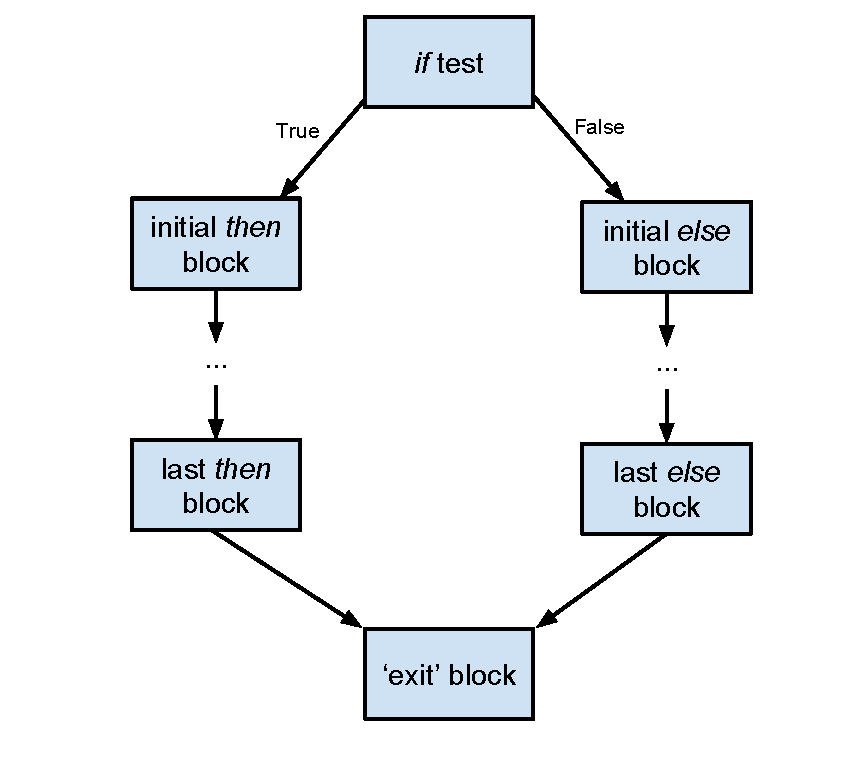
\includegraphics[scale=0.6]{images/cfgIfthenelse.pdf}
        \caption{A general CFG created for \newline an \texttt{if-then-else}.}
    \end{subfigure}% \quad
    \begin{subfigure}[t]{0.5\textwidth}
        \centering
        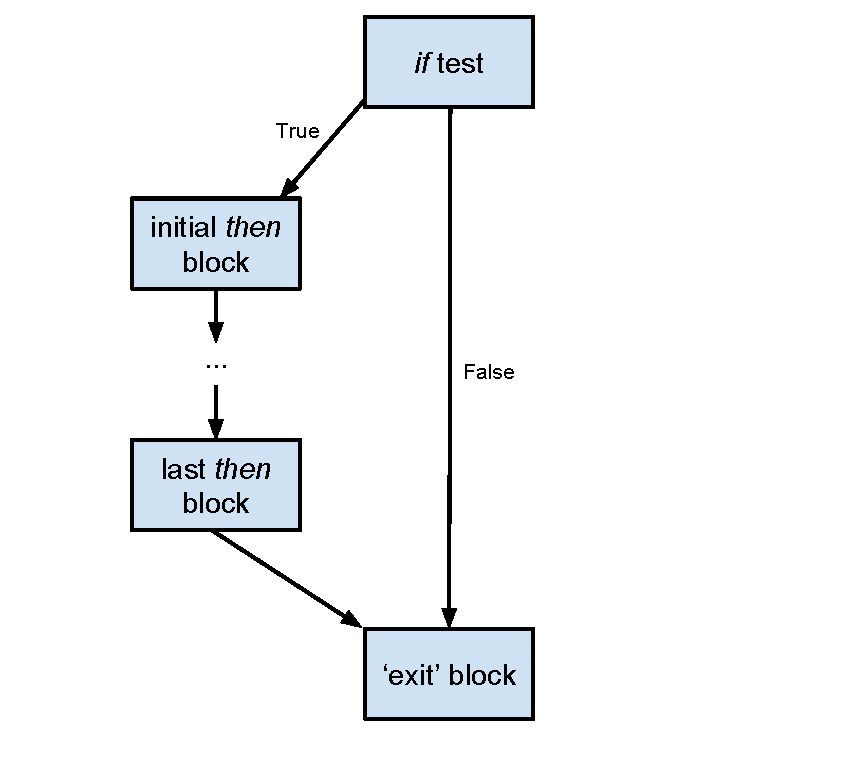
\includegraphics[scale=0.6]{images/cfgIfthen.pdf}
        \caption{A general CFG created for an \texttt{if-then}.}
    \end{subfigure}
    \caption{The cases for CFG generation for \texttt{if} statements.}
    \label{fig:ifcfgs}
\end{figure}



\subsubsection{For and While Loops}
For the purposes of our control flow graph generation, \texttt{for} and \texttt{while} loops are similar and so are dealt with in a similar manner. The process is similar to that of the \texttt{if}.  We create a new block as the initial block for the body of the loop. However, the loop test is given a block to itself and the last block to be active at the end of the loop body is linked the the test block rather than the `exit' block. \\
\indent Python allows an \texttt{else} block to be added the end the loop. An example of this is as follows:
\begin{lstlisting}
    for entry in some_list:
      if entry == thing_i_want_to_find:
        found = entry
        break
    else:
      found = not_found_value
\end{lstlisting}
The \texttt{else} body is always entered if the loop test evaluates to \texttt{False}. In the case of \texttt{for} loops reaching the end of the specified iteration is equivalent to \texttt{False}. The \texttt{else} block is not entered when a \texttt{break}, \texttt{exception} or a \texttt{return} occurs. \\
\indent In the case of an \texttt{else} being present the loop test links to the initial \texttt{else} block and the last block in the \texttt{else} to the `exit' block. Otherwise the test links to the `exit' block. The resulting CFG can be observed in Figure~\ref{fig:loopElseCFG}.

\begin{figure}
\centering
\includegraphics[scale=0.6]{images/loop_else_cfg.pdf}
\caption{The CFG generated for a \texttt{for} loop using an \texttt{else} branch.}
\label{fig:loopElseCFG}
\end{figure}

\paragraph*{Breaks and Continues} \mbox{} \\
In Python, along with most modern languages, a \texttt{break} is used to terminate the inner-most loop and a \texttt{continue} is used to jump to the next iteration of the loop. Taking inspiration from the CFG generation in PyPy, a stack was implemented on which labels are pushed alongside their corresponding nodes. When we reach a loop definition we create a block for the loop `exit' and we push a \texttt{F\_BLOCK\_LOOP} onto the stack. Once we encounter a \texttt{break} or a \texttt{continue} statement we cycle through the labels until we encounter the top-most \texttt{F\_BLOCK\_LOOP} label. Then for a \texttt{break} statement we add an edge between the current block to the loop's `exit' block. For a \texttt{continue} statement we link the current block to the loop head itself. We pop the top of the stack when we finish analysing the loop body. Consider the following function:
\begin{lstlisting}
    def f():
      while some_condition:
        x = 5
        if other_condition:
          break
        else:
          continue
      y = 5.0
\end{lstlisting}
The resulting CFG for this function can be seen in Figure~\ref{fig:whileCFG}. When we encounter the \texttt{while} loop, a \texttt{F\_BLOCK\_LOOP} label along with references to the block containing the loop condition, \texttt{while some\_condition}, as well as a reference to the block containing the loop exit, \texttt{y = 5.0}, is pushed onto the stack. When our analysis encounters the \texttt{break} or \texttt{continue} on line 5 or 7, respectively, we search on the stack for the first instance of an \texttt{F\_BLOCK\_LOOP}. In this case there will only be the single label on the stack. We then extract the reference to the relevant block, the loop exit for \texttt{break} and loop test for \texttt{continue} and set the extracted block as an exit for block containing these statements.

\begin{figure}
    \centering
    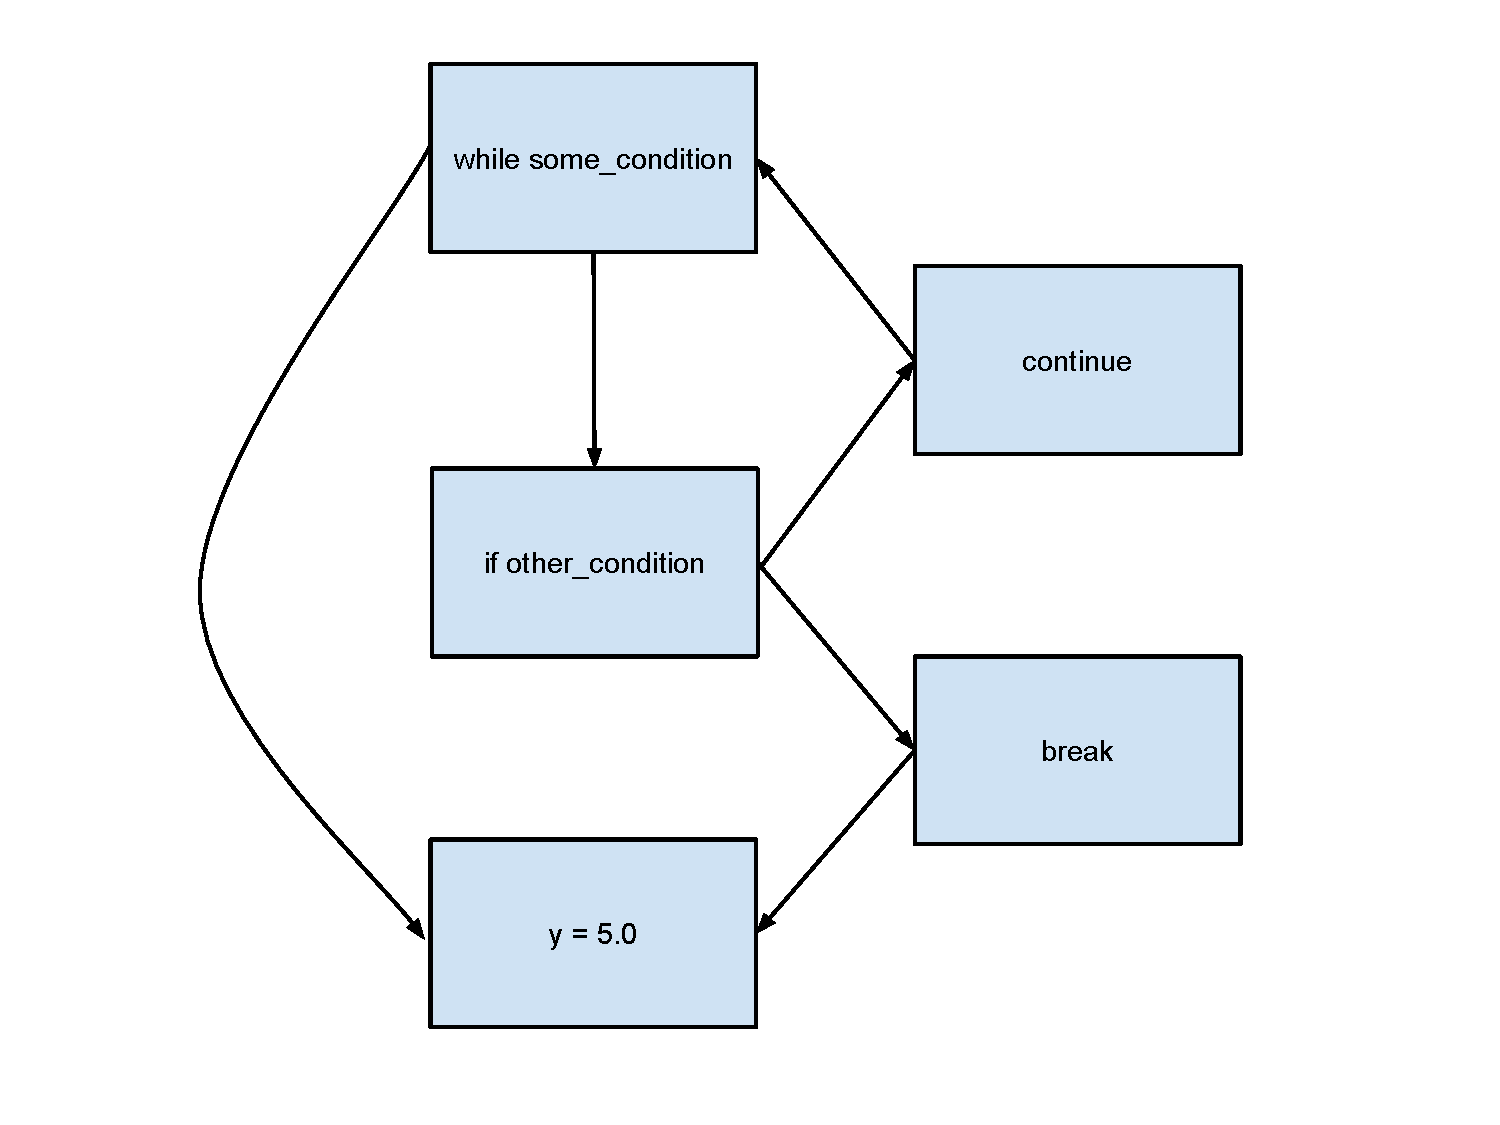
\includegraphics[scale=0.6]{images/whileCFG.pdf}
    \caption{A CFG created for an \texttt{while} loop containing an \texttt{if} with a \texttt{break} in the \texttt{then} body and a \texttt{continue} in the \texttt{else} body.}
    \label{fig:whileCFG}
\end{figure}

\subsubsection{Try, Except and Finally}
The \texttt{try} keyword can be used in a few different ways in Python. Firstly, it can be used as part of a \texttt{try}/\texttt{except} block to handle exceptions, much like \texttt{try}/\texttt{catch} blocks in Java. Also like in Java, different exceptions in the same \texttt{try} block can be caught and dealt with separately. Consider the following example:
\begin{lstlisting}
    try:
      if some_condition:
        open("myfile.txt")
      else:
        x = 5 / y        
    except IOError:
      # Deal with error
    except ZeroDivisionError:
      # Deal with error
\end{lstlisting}
The statement \texttt{open("myfile.txt")} will raise an \texttt{IOError} exception if, for instance, the file does not exist. The \texttt{x = 5 / y} will raise an \texttt{ZeroDivisionError} if \texttt{y} is equal to \texttt{0} at the time of execution. The matching \texttt{except} block will be executed in the case one of the exceptions is raised. In order to accurately create a control flow graph for \texttt{try} and \texttt{except}s we need to know which statements can create exceptions and which exceptions they can create. While very time consuming, this knowledge can be gathered from the built-in exceptions and statements in the Python language and standard library and then hardcoded into our CFG generator. But Python permits the creation of unique exceptions by creating a class which inherits from the built-in \texttt{Exception} class. This would be very difficult to track. For this reason the design decision was made to attempt to minimise any false positives which may result from not creating an edge from potentially exceptional statements to their corresponding \texttt{except} blocks. This was done by determining that every statement in a \texttt{try} block can lead to every \texttt{except} block. This method results in an over-approximation of the possible paths taken inside of the \texttt{try} block. The CFG generated for the above example can be observed in Figure~\ref{fig:tryExceptCFG}. \\

\begin{figure}
    \centering
    \includegraphics[scale=0.6]{images/tryExceptCFG.pdf}
    \caption{A CFG created for an \texttt{try}/\texttt{except} block. All statements in the \texttt{try} has an edge with each \texttt{except} block. The `exit' block has been left out for simplicity.}
    \label{fig:tryExceptCFG}
\end{figure}

\indent Another application of \texttt{try} is to ensure that a particular block of code is unconditionally executed. This is done by using the \texttt{finally} keyword. All code in the \texttt{finally} block is executed no matter how the \texttt{try} body is exited. Normally \texttt{finally}s are used for clean up code. For example:
\begin{lstlisting}
    try:
      file = open(filePath, 'w')
      file.write("something")
    finally:
      file.close()
\end{lstlisting}
\indent Nested \texttt{finally}s are all executed no matter where an \texttt{exception}, \texttt{return} or \texttt{break} occurs. For instance if the following is executed:
\begin{lstlisting}
    try:
      x = 1
      try:
        return
      finally:
        print("finally 1")
    finally:
      print("finally 2")
\end{lstlisting}
Then ``finally 1'' and ``finally 2'' will be printed in that order. \\
\indent The keywords \texttt{finally} and \texttt{except} can be simultaneously used with a \texttt{try}. In this case the relevant \texttt{except} block is executed first and then passes control to the finally block. \\
\indent If a \texttt{try}/\texttt{finally} is within a \texttt{try}/\texttt{except} then exceptions raised still lead to the \texttt{finally} before passing control to the outer \texttt{except} block. For example:
\begin{lstlisting}
    try:
      x = 1
      try:
        raise Exception
      finally:
        print("finally")
    except:
      print("except")
\end{lstlisting}
In the above example after the exception is raised then ``finally'' and ``except'' are printed in that order. \\
\indent Python provides a way for the \texttt{else} keyword to be used in conjunction with \texttt{try}s. The \texttt{else} block is executed after the \texttt{try} body providing no exception is raised. This is typically used in cases where one action is to be taken for exceptional execution and another for non-exceptional execution. For example:
\begin{lstlisting}
    try:
      result = 1 / f(x)
    except ZeroDivisionError:
      logging.info('Infinite result')
    else:
      logging.info('Finite result')
\end{lstlisting}
When an \texttt{else} is used in conjunction with a \texttt{finally} then the \texttt{else} body is executed before the body of the \texttt{finally}. \\
\indent It is illegal for a \texttt{continue} statement to be inside of \texttt{finally} block. This will be detected in the CFG generation. An error regarding this will be printed and the program will terminate. \\
\indent The \texttt{break} and \texttt{continue} statements are illegal outside of a loop. However, unlike a \texttt{continue} inside of a \texttt{finally} block, this does not damage the integrity of the CFG. For this reason an error is printed and processing is continued. \\
\indent If a \texttt{break}, \texttt{return} or \texttt{continue} occurs inside of the \texttt{try} body of a \texttt{try}/\texttt{finally}, control is transferred to the \texttt{finally} block before being transferred to the end of the loop for a \texttt{break}, the end of the function for a \texttt{return} and the loop test for a \texttt{continue}. For this reason, similar to loops, we push a \texttt{F\_BLOCK\_FINALLY} onto our stack when we analyse the \texttt{try} body of a \texttt{try}/\texttt{finally}. The stack is checked for a \texttt{F\_BLOCK\_FINALLY} when we encounter a \texttt{break}, \texttt{return} or \texttt{continue}. If one is found then we set an edge between the block containing the keyword and the \texttt{finally} block. An edge is also set between the \texttt{finally} block and the appropriate destination for the given keyword.



\subsubsection{Merging Empty Exit Blocks}
At the end of the programming constructs dictating control flow, a new block is created as an `exit' block to which the blocks exiting the construct (such as a \texttt{break} in a loop) are linked. However, redundant blocks are generated when constructs are nested. Consider the following:
\begin{lstlisting}
    if c1:
      # First then block
      if c2:
        # Second then block
      else:
        # second else block
    else:
      # Second else block
    # exit
\end{lstlisting}
The exit block for the inner \texttt{if} is not needed as there are no further statements in the first \texttt{then} body. Instead the exit block for the inner \texttt{if} should be the same as the outer \texttt{if} as exiting each one will lead to the same block. Thus we need to merge the inner exit with the outer. To ensure this occurs we check the last active block once each path has been analysed. If the block is not empty then we proceed as normal. If the block is empty we delete the block and update the reference to point to the exit block for the current construct.

\subsection{SSA Form}
The implementation of SSA renaming was performed as described in the background section. However, a few Python specific additions were necessary which are described in this section. \\
\indent Having created the CFG, our SSA renaming can ignore specific programming constructs such as \texttt{for}, \texttt{if} and \texttt{while}. The knowledge required to successfully create the $\phi$ functions for these constructs is encapsulated in the CFG. \\
\indent The algorithm works by analysing one function at a time. A dictionary is maintained with each variable name eligible within the current scope. The dictionary is reset to containing only module/class wide variables at the end of each function. When a identifier is encountered it is determined whether we wish to rename it. If we do then we check whether it is a \texttt{store} or \texttt{load} operation. A \texttt{store} checks whether the identifier has been referenced beforehand. If it hasn't we add the identifier to the dictionary along with the value \texttt{1} and we modify the node containing the variable name by appending that value to the end of the name, so, for instance, \texttt{x} becomes \texttt{x1}. Otherwise the identifier's value is incremented and renamed with the new value. A \texttt{load} operation uses the latest value for that identifier for renaming. Once we reach the end of a basic block the state of current block's dictionary is forwarded to all of the block's successors.

\subsubsection{Global and Local Variables}
\label{chap:ssaGlobals}
We consider a global variable to be a variable in the module-wide or class-wide namespace. This includes all imports, function identifiers and all of the built-in functions and classes. A local variable is one which is limited to the scope of a function. \\
\indent Consider the following snippet of Python code:
\begin{lstlisting}
    class C():
      def f(self):
        self.x = 5
     
      def g(self):
        self.x = 5.0         
        
      def h(self):
        a + self.x 
\end{lstlisting}
The references to \texttt{self.x} refer to the same variable. The principles of SSA naming state that a variable should only be assigned to once. But which \texttt{x} should be labelled \texttt{x1} and which should be labelled \texttt{x2}? Or, rather, which of the assignments to \texttt{x} in function \texttt{f} and function \texttt{g} will be called first? Without any analysis of the call sites or typical run-time behaviour it is impossible to determine this statically. A similar problem arises when we attempt to decide which reference to give to the instance of \texttt{self.x} in function \texttt{h}. Without knowledge of the order the functions are called (if a consistent ordering even exists) we cannot predict which is the correct label. For this reason SSA naming is only performed on local variables. \\
\indent Separating which variables are global and which are local is not simple due to the fact it can change line-by-line.

\paragraph*{The \texttt{global} Keyword}\mbox{} \\
The keyword \texttt{global} is used in Python to enable the programmer to write to the global namespace within a function. By default the programmer has immediate read access to the global scope and read/write access to the local scope. This means the \texttt{global} keyword is only necessary when a write to the global scope is to take place within a function. With the \texttt{global} keyword global variables can be defined dynamically at runtime. If an attempt is made to modify a global variable without specifying the variable as global, then a local variable with the same name is created instead. Consider the following code:
\begin{lstlisting}
    x =  5
    def f():
      x = "Hi"
      y = x
      
      
    def g():
      global x
      x = 5.0
      y = x
\end{lstlisting}
Function \texttt{f} does not modify the global variable. Instead a local variable is created which masks the global variable \texttt{x} from the scope. In the rest of the function \texttt{x} will reference the local variable created. The global \texttt{x} cannot be accessed unless a highly dynamic method is used, such as \texttt{globals().get("x")} where the function \texttt{globals} returns a dictionary containing all global variables. \\
\indent It is common in Python to use the \texttt{global} keyword at the beginning of a function to increase clarity, however Python code in which the global keyword is used \textit{after} the variable has been assigned functions correctly, i.e.\ \texttt{x} in the global namespace is assigned the value (despite the Python interpreter issuing a warning to the programmer.) Therefore we need to be careful if the variable name is used in conjunction with the keyword \textit{somewhere} in the function. \\
\indent Using this knowledge, every time a global variable is modified inside a function we begin the SSA naming unless the identifier is inside of a list of variables which are used in conjunction with the \texttt{global} keyword at some point in the function. For example:
\begin{lstlisting}
    # Set x to be a module-wide global
    x =  5
    
    def f():
      y = x
      x1 = "Hi"
      y = x1
      
     
    def g():
      global x
      x = 5.0
      y = x
\end{lstlisting}
In function \texttt{f} the global keyword is not used with \texttt{x} and so we perform SSA on the variable whereas in function \texttt{g} it has been used and so the identifier is not renamed.

\subsubsection{Generating $\phi$ Functions}
Two methods for generating $\phi$ functions were described in the background section. These were: to calculate dominance frontiers, or to naively place them for all variables at the beginning of each block. The decision was made to implement the naive approach. This decision was taken as we felt it was more important, and interesting, to cover more of the Python language rather than to increase the speed of the tool. We currently generate $\phi$ functions for all local variables within a function.

\subsection{Type Inference}
Type inference in our system works by creating a network modelling the data flow of types. The inference works by propagating primitive types through constraints until the system has been completely satisfied. \\
\indent A thorough description of all of Python's built-in types can be found~\cite{pythonTypeDocs}. The types supported by our tool are:
\begin{itemize}
	\item \texttt{int} - a numeric type to represent an integer. It has unlimited precision.
	\item \texttt{float} - a numeric type to represent a floating-point number.
	\item \texttt{bool} - a subtype of \texttt{int}. Used in comparisons.
	\item \texttt{bytes} - a sequence of integers.
	\item \texttt{string} - stores a sequences of Unicode code characters. There is no distinction for single characters.
	\item \texttt{list} - a type used to store sequences of items.
	\item \texttt{tuple} - a type used to store sequences of items.
	\item \texttt{dict} - a type used to store (key, value) pairs.
	\item \texttt{set} - a type used to store unordered collection of distinct hashable objects.
	\item \texttt{generator} - a type used to provide an iterator over a sequence. Each item is deleted from the iterator after it has been visited.
	\item \texttt{none} - represents the \texttt{None} type in Python.
	\item \texttt{module} - a type representing modules as well as packages.
	\item \texttt{class definition} - a type which represents an uninstantiated definition of a class.
	\item \texttt{class instance} - a type which represents an instantiation of a class definition
	\item \texttt{function} - a type representing a function.
\end{itemize}
The built-in types not supported by our tool are \texttt{bytearray} and \texttt{complex}. However, from our experience, they are not very common.

\subsubsection{Built-in Functions}
\indent All built-in types but \texttt{int} and \texttt{float} have functions as class members which can be called from instances of these types. Almost all of these are supported. In total, across all built-in types, 177 functions are supported at the time of writing. For brevity they have not be been documented here. For a significant number of these functions, the information necessary to support them in our tool was extracted from mypy~\cite{mypy}. \\
\indent Python provides a number of polymorphic built-in functions. For example, \texttt{abs} takes a single numeric parameter, an \texttt{int} or a \texttt{float}, and returns the absolute value of that number. At the time of writing, 53 built-in functions are supported which covers the most frequently used functions. Again, for brevity they have not be been documented here. \\
\indent In addition to the above types we make use of a type not found Python, \texttt{any}, which represents the fact the variable could be any possible type and as such is permitted in all circumstances. \\
\indent Initially a pass over the entire program is made and every variable encountered is initialised to an empty set of types. Each context in the program has a mapping from the name of every variable accessible in the current scope to its corresponding type variable. In the case that access to the variable is permitted in more than one scope, such as module-wide global in a function, the corresponding type variable is passed from the parent context to the child.

\subsubsection{Inferring the Types of Simple Assignments}
All changes to the types of variables involve assignments. For each assignment the variable on the left-hand side (LHS) assumes all of the types which the right-hand side (RHS) can possibly have. The following shows a number of ways in which this can be done.
\begin{lstlisting}
	x = 5
	y = x
	z = f()
\end{lstlisting}
 If the RHS is a function then we assign all of the types the function can possibly return. \\
\indent We simulate this flow of types with a simple subset relationship. The set of types the RHS can assume must be a subset of the set of types the LHS can assume. An example of this can be observed in Figure~\ref{fig:assignConstraint}. \\
\indent Python allows assignment to variables to be performed inside of \texttt{list}s or \texttt{tuple}s. For example:
\begin{lstlisting}
    (x, y) = (1, 1.0)   # 1
    [x, y] = [1, 1.0]   # 2
         x = (1, 1.0)   # 3
         x = [1, 1.0]   # 4
\end{lstlisting}
In the first and second cases \texttt{x} is assigned an \texttt{int} type and \texttt{y} is assigned a \texttt{float} type. However in the third and fourth cases we want to assign a \texttt{tuple} and \texttt{list} type to \texttt{x} respectively. \\
\indent Python also supports double assignment such as the following:
\begin{lstlisting}
    x = y = 5
\end{lstlisting}
This is equivalent to \texttt{x = 5; y = 5} rather than \texttt{x = 5; y = x}. For local variables we would not be able to distinguish the difference. However for global variables this would result in an over-approximation. For example, if \texttt{x} was a global variable then it may already contain types other than \texttt{int} and so \texttt{y} would be assigned types it could never obtain.

\begin{figure}
\centering
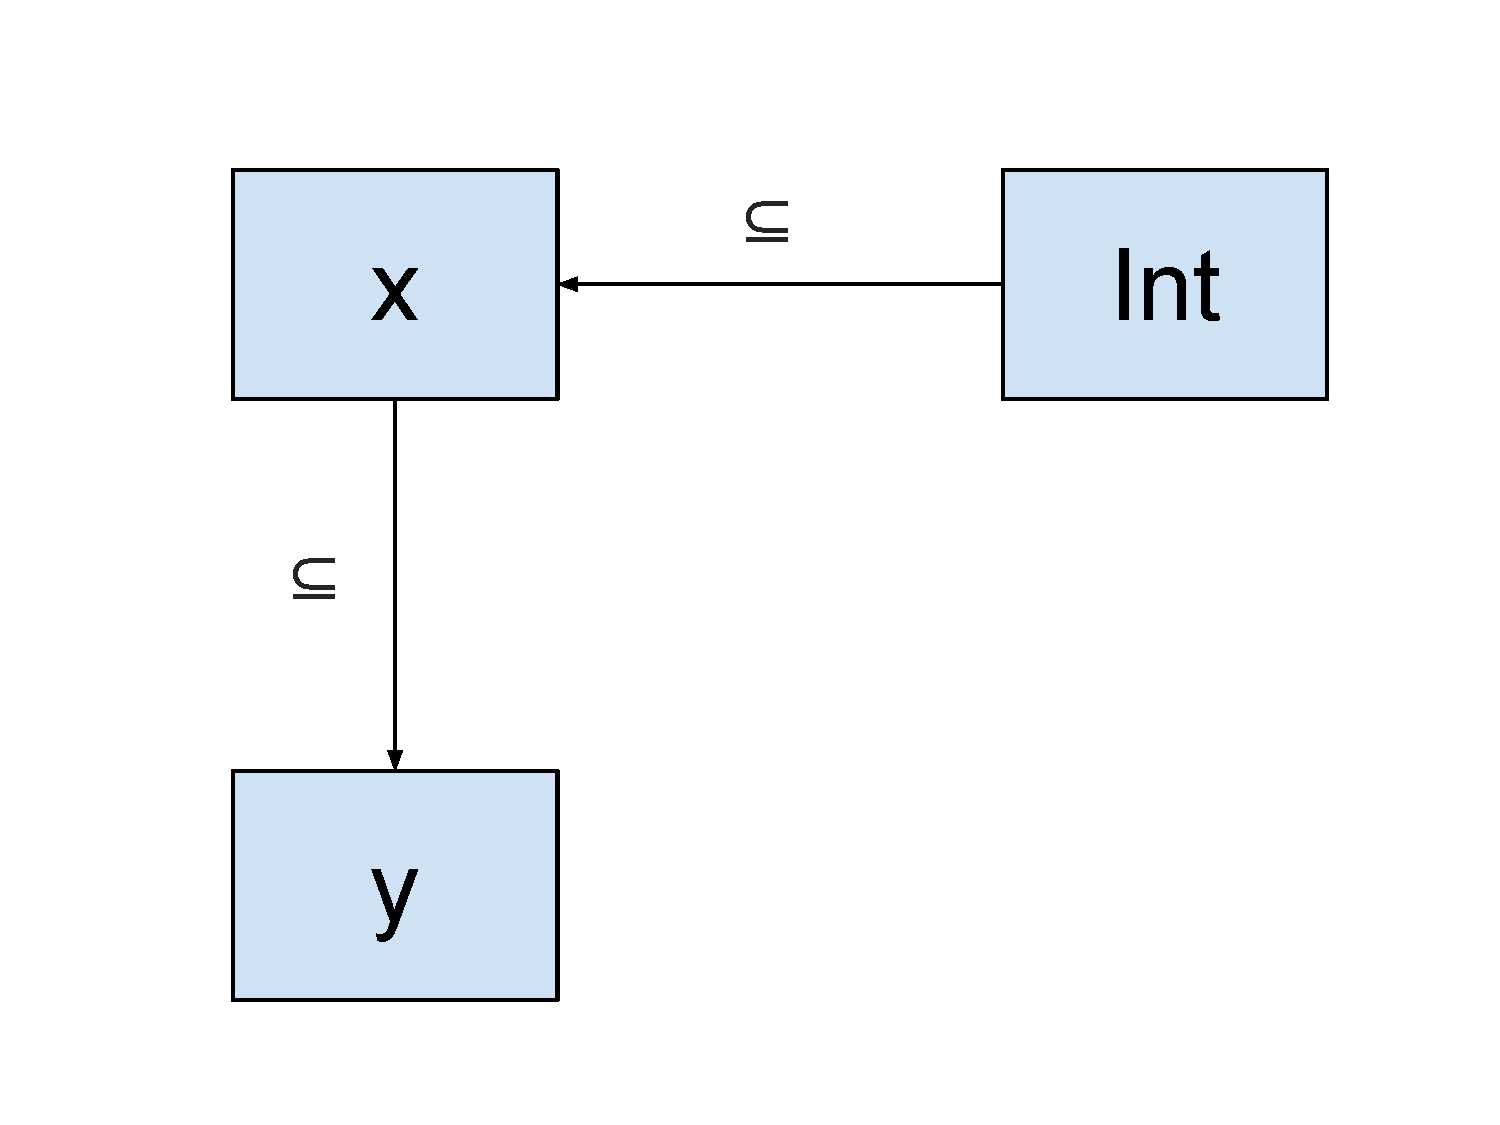
\includegraphics[scale=0.3]{images/assignment_constraint.pdf}
\caption{The network generated by the assignments, \texttt{x = 5} and \texttt{y = x}.}
\label{fig:assignConstraint}
\end{figure}

\subsubsection{Inferring the Types of Binary Operations}
Binary operators are handled by our type inferencer by first inferring the types of the left and right hand side of the operator. We then determine whether there is at least one combination between the two sets of types which can be legally used with the operator. \\
\indent A comprehensive list of the binary operators and the types which can be legally used in combination with them can be seen in Appendix~\ref{App:AppendixBinary}.


\subsubsection{Inferring the Types of Unary Assignments}
Python has a small number of unary operators. These are all numeric operators, such as the bitwise not, $\sim$, aside from the boolean operator \texttt{not}. The numeric operators can only be applied to \texttt{ints} and \texttt{floats} and will return the same numeric type. However the \texttt{not} operator can be legally applied to any type and will always return the type \texttt{bool}.

\subsubsection{Inferring the Types in a `Container' Type}
\label{chap:inferringContainers}
By a `container' we refer to any type which can contain a sequence of other types. Built-in containers are \texttt{list}, \texttt{dict}, \texttt{set}, \texttt{generator} and \texttt{tuple}. \\
\indent New elements can be added to these container typically through indexing and using functions. For example, using a list:
\begin{lstlisting}
    x = []
    x[0] = 5        # Indexing
    x.append(5.0)   # Using a function
\end{lstlisting}
No container in Python is restricted to elements of any one type. In the example above the elements of \texttt{list} \texttt{x} are of type \texttt{int} and \texttt{float} after the function \texttt{append} has been called. In the case of a \texttt{dict}, which is a mapping of key/values pairs, it is not limited in the types it contains for keys or values. For instance a single \texttt{dict} instance could contains mappings from \texttt{strings} to \texttt{ints} and \texttt{floats} to \texttt{lists}. \\
\indent All of these container types, aside from \texttt{tuple}, are \textit{mutable}. A type is mutable if the value of an instance of the type is liable to change. The value of an instance of an \textit{immutable} type is not liable to change to chance once it is created~\cite{pythonMutable}. The effect of this is the following:
\begin{lstlisting}
    def f(y):
      y.append("mutable")
     
    def g(y):
      y = 5.0
      
    x = [5]
    f(x)
    print(x)    # prints [5, "mutable"]
    
    x = 5
    g(x)
    print(x)    # prints 5
\end{lstlisting}
The \texttt{int} type is immutable and so the function \texttt{g} can in no way edit the value of the \texttt{int} object. Since the \texttt{list} is mutable the function call to \texttt{f} on line 8 was able to change the contents of the list and therefore the types of the elements contained in the list. What this means in the context of the type checking is that if we wish to accurately track the possible types of the contents of a container type then we must also keep track of the possible side-effects of functions. In the case above we must express that the function \texttt{f} will always add the type \texttt{string} to its first (and only) parameter. When the function is called we must update the possible types the elements of the \texttt{list} can contain. So, for example:
\begin{lstlisting}
    def g():
      x1 = [3]
      f(x1)
      x2 = __side_effects(f, x1)
      print(x2)
\end{lstlisting}
where \texttt{\_\_side\_effects} performs whatever the changes the function has on the contents of \texttt{x1}. The type of \texttt{x1} may need to be updated due to the changes that \texttt{f} may have on the contents of \texttt{x1}. The same must also be done for the built-in functions, such as \texttt{append} for \texttt{list} which adds the parameter to the list. \\
\indent Unfortunately this process is either all-or-nothing. Performing type inference only in some cases, such as only indexing would cause our tool to return false-positives. For example, if we encounter the following two statements: \texttt{some\_list[i] = 5; some\_list.append("hi")} only accepting new types from indexing would give \texttt{some\_list} the type \texttt{\{int\}} when in fact it should have type \texttt{\{int, string\}}. If an item is then taken from the list and used in a function which accepts only the \texttt{string} type then a false positive will occur. Due to this and the time and difficulty in calculating the side-effects of functions we consider the contents of a container to always be of type \texttt{any}.

\subsubsection{Inferring the Types in del Statements}
\label{chap:del}
The \texttt{del} statement is used to remove an identifier binding. If the target of the \texttt{del}  statement is a variable then the type of that variable is set to the Python type \texttt{None}. Otherwise, if the target is an element of a list or \texttt{dict} then that single element is removed. In the case of a variable we can change the type assigned to this variable to \texttt{none}. In the case that the target is an element of a container we do nothing. Since we do not track the types in a container we are able to ignore this operation.

\subsubsection{Inferring the Types in If Expressions}
Python allows the \texttt{if} keyword to be used in expressions. These expressions are typically used to conditionally assign values to a variable. For example: \texttt{x = 5 if some\_condition else "Hi"}. In the case that \texttt{some\_condition} evaluates to true then \texttt{x} is assigned the value \texttt{5}, otherwise \texttt{x} is assigned the value \texttt{"Hi"}. No attempts are made to determine the likely path taken by the \texttt{if} condition and so we set the resulting type of the \texttt{if} expression to the type of the union of the \texttt{then} branch and the \texttt{else} branch.

\subsubsection{Inferring the Types in Comprehensions}
Python provides convenient syntax for generating a number of different container types, such as \texttt{list}, \texttt{dict} and \texttt{generator}. These are called comprehensions. For example, assume we have a Python \texttt{list}, \texttt{num\_list}, containing various \texttt{int}s and we wished to extract all numbers of a value less than 100 into a new \texttt{list}. We could do this using the following \texttt{list} comprehension: \texttt{[x < 100 for x in num\_list]}. The \texttt{for x in some\_list} generates an iterator over all values in \texttt{num\_list} and assigns each value to the variable \texttt{x}. Each value is then added to a new \texttt{list} if the condition \texttt{x < 100} evaluates to true for that value. \\
\indent Each of the comprehensions are performed in similar ways but are differentiated by the syntax which surrounds the expression. \texttt{list} comprehensions use \texttt{[expr]} as above, \texttt{dict} comprehensions use \texttt{\{expr\}} and \texttt{generator} comprehensions use \texttt{(expr)}. \\
\indent In each comprehension the return type is the type of comprehension, e.g.\ a \texttt{list} comprehension always returns a \texttt{list} type.

\subsubsection{Inferring the Types in For/While Loops}
The following shows a `raw' while loop and the same while loop in SSA form:
\begin{lstlisting}[mathescape]
    # Raw form
    x = 5
    while (p):
      y = x
      x = "Hi"
	
    # SSA form
    x1 = 5
    while (x2 = $\phi$(x1, x3), y2 = $\phi$(y1) p):
      y1 = x2
      x3 = "Hi"
\end{lstlisting}
A problem raised by this is that the $\phi$ function at the beginning of the loop depends on the types which can not be determined until the end of the loop body. In between there may be other variables which use the result of the $\phi$ function in their own assignment, like \texttt{y1} above. Due to the manner we deal with simple assignment, using the subset relation, we can treat the $\phi$ function as a number of different assignments to the variable created by the $\phi$ function. So, for example, \texttt{x2 = $\phi$(x1, x3)} would translate to $\mathtt{x2 \subseteq x1}$ and $\mathtt{x2 \subseteq x3}$. Thus, while in the example above \texttt{x3} may be an empty type variable once we set up the relationship the types will flow through to \texttt{x4} as \texttt{x3} receives them. \\
\indent We need to consider what types can be legally used in the loop tests. The case for \texttt{while} loop tests require no significant effort since any type can be compared to a boolean value, however \texttt{for} loops use the Python concept of \texttt{iterators}. \texttt{iterators} work by systematically yielding each object that they contain until all objects have been exhausted. \\
\indent A Python type qualifies as an iterator if it implements the \texttt{\_\_iter\_\_} function. The built-in types which implement \texttt{\_\_iter\_\_} are \texttt{list}, \texttt{sting}, \texttt{tuple}, \texttt{dict} and \texttt{set}. Therefore, when we encounter a \texttt{for} loop we check whether the iterator used implements the \texttt{\_\_iter\_\_} function.


\subsubsection{Inferring the Possible Types of Function Arguments}
\label{chap:inferringFuncArgs}
There are a number of different types of arguments in Python. These are:
\begin{itemize}
	\item Regular function arguments
	\item Default function arguments
	\item Variable-length function arguments
	\item Keyword function arguments
\end{itemize}
We will briefly discuss each of these and how we deal with them.

\paragraph*{Regular Function Arguments}\mbox{} \\
Regular function arguments work in largely the same way as in C and Java. All regular function arguments are required to be given a value when the function is called. A regular argument is signified in the function definition by listing the identifier of the argument only. For example, \texttt{def f(x, y)} is a function header with regular arguments only.

\paragraph*{Default Function Arguments}\mbox{} \\
A default argument is similar to a regular function argument apart from the fact it doesn't need to be given a value when the function is called. When the argument is not given a value, it takes on a default value which is specified in the function header. For example, the function header \texttt{def f(x, y = 2.0)} has \texttt{x} as regular function argument and \texttt{y} as default argument with a default value of \texttt{2.0}. This function can be called in the following styles: \texttt{f(1, 1.0)}, \texttt{f(1)}. In the first case the argument \texttt{y} takes on the value of \texttt{1.0} as given, but in the second case the \texttt{y} takes on the default value of \texttt{2.0}. \\
\indent Any number of default arguments can be given, however they must succeed all regular function arguments. The header \texttt{def f(x, y = 1.0, z)} is illegal. This error is caught by the AST parser and so we do not have to consider it. \\
\indent Default arguments are the most common of the `special' function arguments. We consider them only during function calls. We record the number of default arguments and allow the function call to be short of a maximum of that many arguments. We do not use the default value in our type inference since the type may well be incorrect.

\paragraph*{Variable-length Function Arguments}\mbox{} \\
Variable-length function arguments, or \textit{varargs}, are used to allow a function call to provide an unbounded number of arguments. A vararg is signified by preceding the identifier with a \texttt{*}. For example, the function header \texttt{def f(x, *y)} has a regular argument and a vararg. Similarly to the default argument, the vararg does not need to be given a value in a function call. The type of the vararg is always a \texttt{tuple} and will contain all arguments given after the required arguments and default arguments. For example, the call \texttt{f(1, 2, 3, "hi")} will give the parameter \texttt{y} the \texttt{tuple} \texttt{(2, 3, "hi")}. \\
\indent varargs are not very common. In the library functions we have supported in our system they have occurred 7 times out of the 230 built-in functions supported by our tool. However, not supporting varargs does not raise any false positives. Since the type of a vararg is always \texttt{tuple} we can type the function argument accurately. The only downside is that the cannot type check the parameters in a function call to a function using varargs. 

\paragraph*{Keyword Function Arguments}\mbox{} \\
Keyword function arguments, or \textit{kwargs}, are similar to varargs in that they allow unbounded number of arguments to be given to the function call. A kwarg is signified by preceding the identifier with \texttt{**}. For example, the function header \texttt{def f(x, **y)} has a regular argument and a kwarg. The difference between a kwarg and a vararg is that an identifier needs to be provided along with each value. Each identifier and value pair is provided in a \texttt{dict}. For example, the function call \texttt{f(5, item1 = 1, item2 = 2)} will cause \texttt{y} to take on the \texttt{dict} \texttt{\{item1 : 1, item2 : 2\}}. \\
\indent kwargs are the least common `special' function argument. They are used only twice in our supported library functions. For this reason they are also not type checked. Similarly to varargs the kwargs only ever assume one type. Due to this we can always type the kwarg as a \texttt{dict}. However, again, we unable to check the correct parameter types are given to the call of a function using kwargs. \\
\indent Keyword function arguments can be used without the \texttt{**} syntax by referring to the function arguments in the function call by the name they are given in the function header. This allows the function arguments to given out-of-order. For example, the function with the header \texttt{def f(x, y)} can be called in the following way: \texttt{f(y = 4, x = 5)}. Currently, this method of calling functions is not supported. \\



There are two different methods of inferring the types of function arguments we can consider. We could use either a \textit{top-down} approach or a \textit{bottom-up} approach.

\paragraph*{Top-Down: Extracting Information From Call Sites}\mbox{} \\
A top-down approach involves finding all of the calls to a function and determining the types the function accepts by inferring the types of the values given to the function. This means we assume all of the values to be correct. The benefits to this approach are that the return types inferred for the functions should be quire accurate since there will be no function, which has been called in the source code, with arguments typed as \texttt{any}. However there are two major downsides. Firstly, we lose a bug-checking opportunity at all call sites. We rely on the types given to the function call to be valid. Secondly, any errors which may be present at the call site will propagate through the function call body. Any clashes with the types used in the function body will result in an error being reported in the wrong place. For example, consider the following code in which a function is called with the wrong type:
\begin{lstlisting}[mathescape]
    def add_one(x):
      return x + 1    	
    	
    # Only call to function f
    add_one("Hi")
\end{lstlisting}
Analysing the given code with a top-down approach would see that the only the function call to \texttt{add\_one} gives the argument \texttt{x} a \texttt{string} type thus giving the argument a type set containing only \texttt{string}. Due to this an error will be flagged on the use of the \texttt{int} \texttt{1} in a binary \texttt{+} operation with \texttt{x}. While an error will certainly occur at that line when the function is called with a string, the line \texttt{x + 1} is not the cause of error but instead the function call. In this case, assuming that the types given to function calls are correct is not a reasonable assumption and will cause the type checker to raise errors in the wrong places.

\paragraph*{Bottom-Up: Extracting Information From Parameter Use}\mbox{} \\
A bottom-up approach involves determining the types of arguments solely by how they are used within the function body. To do this we make use of pre-existing knowledge from the types which other functions and built-in operators accept. If a parameter is used within a context then the types that parameter can take are changed to the types applicable in that context. \\

It was felt that more was to be gained using the bottom-up approach since we would be able to detect errors caused by incorrect types being passed to a function. It is important to note that useful information can be extracted from the calls. There is a possibility of using this information when we are unable to infer the types of the parameters using the function body in isolation. However this is currently not done. \\
\indent To implement this approach we observe how each parameter is used and what possible types that it can legally assume in these contexts. When we are unable to infer any useful context in which the parameter is used, we resort to labelling the parameter as having \texttt{any} type. \\
\indent We observe the following contexts to infer types for parameters:
\begin{itemize}
	\item Whether the parameter is indexed
	\item Whether the parameter is used in a binary operation
	\item Whether the parameter is iterated over
\end{itemize}
In each case we use the types which are legally allowed in each operation to infer the types for the parameter. \\
\indent We do not currently use whether the parameter is called to infer the types, e.g.\ if \texttt{x} is parameter and used in the following way: \texttt{x()}. This is because any function, class definition or class instance which implements \texttt{\_\_call\_\_} can satisfy this context. There are hundreds of built-in functions and classes which it could possibly be and cataloguing all of these would take more time than it is worth. \\
\indent There are times when the same context of the parameter should be used differently. Consider the following two functions:
\begin{lstlisting}[mathescape]
	def f(x, y):
	  return x + y
		
	def g(x, y):
	  if (p1):
	    return x + y
	  return 0
\end{lstlisting}
Both functions apply the \texttt{+} operator to the parameters. However, due to the \texttt{if} statement the constraint this imposes on the types they can take is quite different. In function \texttt{f} the operation is unconditional and so we know that both parameters are required to be of a type (or a sub-type of a type) which can used in this operation. On the other hand, in the function \texttt{g} this statement may not be executed in which case we can see that no type errors can occur. This leads us to conclude that we must take the context of the statement into account before we issue a constraint.

\subsubsection{Inferring the Possible Return Types of a Function}
To infer return types, we simply create a type variable to represent the return type of the function, $\alpha$. For every \texttt{return} statement we come across we create a subset relationship between the value of the return statement and our type variable. For example:
\begin{lstlisting}[mathescape]
    def f():
      if (p1):
        return 5
      if (p2):
        return "Hi"
      return
\end{lstlisting}
Here we create the subset relationships $\texttt{int} \subseteq \alpha$, $\texttt{string} \subseteq \alpha$, $\texttt{none} \subseteq \alpha$ which would result in $\alpha$ assuming the type set $\{\texttt{int}, \texttt{string}, \texttt{none}\}$. \\
\indent There is the possibility of a relationship between the types of the parameters and the return types, e.g.\ a string is always returned if an integer is given. While this addition would improve the accuracy of our type inference, it would be complex to implement and so we currently do not do this.

\subsubsection{Generator Functions and the \texttt{yield} Keyword}
The \texttt{generator} type is an iterator which lazily generates values to be iterated over. Functions which return a \texttt{generator} type use the \texttt{yield} keyword in place of \texttt{return}. For example:
\begin{lstlisting}[mathescape]
    def f():
      for x in range(10):
        yield x + 1
    
    for x in f():
      print(x)
\end{lstlisting}
The function \texttt{f} returns a \texttt{generator} type which iterates over the values from 1 to 10. When the function \texttt{f} is first called, a \texttt{generator} type is returned and no computation takes place. When the iteration begins on line 6, the function \texttt{f} is entered for the first time and the function body is executed until a \texttt{yield} is reached. The value is returned and computation is paused until another value is required. This continues until the function returns. \\
\indent The types contained in the \texttt{generator} can be inferred by determining all types which can be `yielded'. However since we currently do not track the types in containers we do not do this either. \\
\indent Any function which contains the keyword \texttt{yield} returns a \texttt{generator} type. For instance, despite never being able to reach a \texttt{yield} the following function returns a \texttt{generator} type when first called:
\begin{lstlisting}[mathescape]
    def f():
      return
      yield 6
\end{lstlisting}
For this reason if we encounter a \texttt{yield} keyword contained in a function body we tag the function as a generator function and set the return type of that function to the type \texttt{\{generator\}}.

\subsubsection{Inferring the Types Involving Recursive Functions}
Currently no special measures are taken for recursive functions. However this does not impact on the accuracy in a significant way. Consider the following recursive function in Python for calculating factorials:
\begin{lstlisting}[mathescape]
    def factorial(n):
      if n == 1:
        return 1
      else:
        return n * factorial(n-1)
\end{lstlisting}
There is enough information in this function to infer the types of the parameter and the return type of the function using our regular method. The base case on line 3, \texttt{return 1}, adds the type \texttt{int} to the return types of the function. The parameter, \texttt{n}, is then used in the multiplication binary operation on line 5. The inferred \texttt{int} return type of the \texttt{factorial} function provides us with enough information to ensure that there is a legal combination of types between the parameter and the return types, of which there are natively two: $\mathtt{int * int}$ and $\mathtt{float * int}$.


\subsubsection{Inferring the Types Contained Within Classes}
\label{chap:inferringClasses}
In statically typed languages such as Java and C++ the class members are required to be specifically defined outside of the function and in the main body of the program. In Python this is not required. The class members which can be accessed outside of a class can be declared in a function within that class, and even outside of the class entirely. If a variable has been declared inside of a function, then the function is required to be called before the variable is referenced. An example of this is as follows:
\begin{lstlisting}[mathescape]
    class C():
      def f():
        self.x = 5
		
      def g():
        self.x = "hi"
        
    # Using the class C
    c = C()
    print(c.x)    # Error
    c.f()
    print(c.x)    # Okay - prints 5
\end{lstlisting}
You may also notice that the class member held by C can be different types - \texttt{int} or \texttt{float} depending on which of the functions \texttt{f} and \texttt{g} was called last. To infer the types of these variables we can use a few different methods.

\paragraph{Method 1: Any Possible Type at Any Time}\mbox{}\\
Whilst analysing the functions of the class we can keep track of all of the possible types of each class member. We do this on a function-by-function basis. So once we have analysed function \texttt{f} we believe that the variable \texttt{x} can be the set of types \texttt{\{int\}}. We update this to \texttt{\{int, float\}} after the analysis of the function \texttt{g}. Once the entire class has been analysed we return all of the possible types a variable can have. This method is not very accurate, and does not take into account the changes that the function calls make to the object.

\paragraph{Method 2: Treat Function Calls as Object Modifiers}\mbox{}\\
Whilst analysing the functions of a class, instead of recording all of the types a variable can take we can tag the function with the variable modifications it makes. So for the example given above we would tag the function \texttt{f} as modifying the variable \texttt{x} to \texttt{\{int\}} and function \texttt{g} as modifying \texttt{x} to \texttt{\{float\}}. However to take advantage of this information we are required to manipulate the calling code somewhat. If we are stating that the functions change the state of the object then we need to explicitly indicate this as we did with `normal' variables with SSA naming. For example, consider the calling code for the class \texttt{C} example we gave above. We would edit this to be something similar to the following:
\begin{lstlisting}[mathescape]
    # Using the class C
    c1 = C()
    print(c1.x)    # Error
    c1.f()
    c2 = $\theta$(c1.f())
    print(c2.x)    # Okay - prints 5
\end{lstlisting}
where the $\theta$ function represents modifications to the class instance (the $\theta$ function is used since the function may return a value.) We assume that the function creates a special kind of assignment to the object with the old object information plus the changes to the global variables made by the function. On top of this we must also take into account the changes the function may perform on variables other than the ones it is called upon. For example, the function may take a class instance as parameter and perform modifications on it. \\
\indent This method is much more accurate than the first as we keep track of how a object instance grows and changes with each function call made upon it. However the price we pay for this accuracy is a much more complex implementation process.

The decision was made to use Method 1. While Method 2 is clearly more accurate, calculating the side-effects of a function would be complicated process and would not fit within the time-scale of the project. \\
\indent To implement Method 1 we treat the class variables in the same manner as we treat module-wide global variables, and so their type is a union of all possible types they can have.


\subsubsection{Inheritance}
In Python a programmer can indicate inheritance by inserting the name of the base class within the parenthesis of the class declaration. This can be seen in the following example:
\begin{lstlisting}[mathescape]
	class C():
	  def f():
	    self.x = 5
		
	  def g():
	    self.x = "hi"

	class D(C):
	  def f():
	    self.y = 5
		
	  def h():
	    self.y = "hi"
\end{lstlisting}
Class \texttt{D} inherits from the base class \texttt{C}. The function \texttt{g} is inherited along with the variable \texttt{x}. Python supports overloading of functions, so the function \texttt{f} inherited from C is overridden by subclass \texttt{D}. \\
\indent Python supports multiple inheritance. This works by separating the base classes with commas in the class declaration. Consider the following example: 
\begin{lstlisting}[mathescape]
	class C():
	  def f():
	    return 4
	    
	class D():
	  def f():
	    return "Hi"
	    
	  def g():
	    self.x = "hi"

	class E(C, D):
	  pass
\end{lstlisting}
When a function is called on a subclass Python initially looks for a declaration in the subclass definition. If it is not found the search is continued through the base classes, in the order they are given, until the referenced identifier is found. Therefore preference is given to the base classes listed first. So, in the previous example, if a call to the function \texttt{f} is made on an instance of class \texttt{E} the search will end at the function instance in class \texttt{C}. \\
\indent We support inheritance by constructing a relationship between the identifiers listed to be inherited from and the subclass being analysed. We need to compile a list of all possible identifiers accessible through the subclass. If an identifier listed in the base class has a class type which can legally be inherited from then all the members in that class, along with their type variables, are inherited by the subclass. \\
\indent A problem arises if we find that a base class has the type \texttt{any}. This most commonly arises when a identifier originating from an un-located import is used (see Chapter~\ref{chap:imports}.) In this case we cannot possibly have any idea which identifiers are inherited. In this case we label the subclass as having an \texttt{any} base type. If any identifier is referenced in the class which is not in the list of global identifiers for the class then we assume it originates from the base class with \texttt{any} type and return the value \texttt{any} type. \\
\indent Python supports dynamic change in the list of base classes through tricks such as the following:
\begin{lstlisting}[mathescape]
CurrentClass = type('CurrentClass', (NewBaseClass,), dict(NewBaseClass.__dict__))
\end{lstlisting}
This behaviour is not supported. For what is likely a rare occurrence and considered `bad coding' by most\footnote{We came to this conclusion since the code is very unreadable. The technique also seems to be taboo on discussion websites, such as: \url{http://stackoverflow.com/questions/9539052/python-dynamically-changing-base-classes-at-runtime-how-to}}, the time required to include support for this dynamic changing of base classes was deemed counter productive to the project as a whole.

\subsubsection{Getting and Setting Attributes}
An attribute is the composition of two identifiers using the \texttt{.}, such as \texttt{x.f}. We will refer to the identifier preceding the \texttt{.}, \texttt{x}, as the \textit{value} and the identifier succeeding the \texttt{.} as the \textit{attr}.  We divide these attributes into two categories:
\begin{itemize}
	\item \textbf{Get} - A load of the attribute, such as \texttt{y = x.f}
	\item \textbf{Set} - A store to the attribute, such as \texttt{x.f = y}
\end{itemize}
In both cases we create a special type variable which carries out the effect of the statement. However the effect they have is different.

\paragraph*{Get Attribute}\mbox{} \\
When we encounter a get attribute we create a \texttt{GetAttributeTypeVariable} which emits the resulting types of the attribute. The \texttt{GetAttributeTypeVariable} is bound to the type variable corresponding to the value of the attribute. For every type that the value can assume the type is tested to see whether it contains a global variable with the same identifier as the attr. A subset relationship is assumed between the \texttt{GetAttributeTypeVariable} and all successfully found global identifiers. The get attribute does not raise any errors providing that at least one global variable matching the identifier from a single type is successfully found.

\paragraph*{Set Attribute}\mbox{} \\
Similarly, for the set attributes we construct a \texttt{SetAttributeTypeVariable}. However we pass it the type variable of the value being passed to the attribute. The \texttt{SetAttributeTypeVariable} is also bound to the type variable corresponding to the value of the attribute. Except for every successfully found attribute we create a subset between the type variable found and the value passed to the \texttt{SetAttributeTypeVariable}. If a type variable matching the attr is not found then one is created and the subset relationship is formed between the new variable and the value. The \texttt{SetAttributeTypeVariable} does not emit any types.


\subsubsection{`Magic' Functions}
Python has a large number of special functions which can be implemented by the programmer which can then be used in a unorthodox way. All of these functions are characterised by having a double leading and trailing underscores. The most frequently used of these are \texttt{\_\_init\_\_} and \texttt{\_\_del\_\_} which act as a constructor and destructor respectively. \\
\indent The functions \texttt{\_\_eq\_\_}, \texttt{\_\_ne\_\_}, \texttt{\_\_gt\_\_}, \texttt{\_\_ge\_\_}, \texttt{\_\_lt\_\_}, \texttt{\_\_le\_\_} are used to define comparisons between objects using the $==$, $\neq$, $\ge$, $\geq$, $<$, $\leq$ operators, respectively. No type errors can ever occur using the $==$, $\neq$, for instance $4 == ``Hi"$ simply returns false. However using the ordering operators, $>$, $\geq$, $<$, $\leq$, on a class which has not defined the respective function results in a type error. \\
\indent There are also `magic' functions for each of the binary operators and an additional one for the augmenting assignment equivalents. Currently, we do not support these particular `magic' functions. \\
\indent We will now discuss the more interesting `magic' functions which are supported.

\paragraph*{The \_\_iter\_\_ Function}\mbox{} \\
The \texttt{\_\_iter\_\_} (short for \textit{iterable} or \textit{iterator}) function defines how an object should be traversed. It is typically used in \texttt{for} loops in the context: \texttt{for item\_name in object\_name}. If an object does not define the \texttt{\_\_iter\_\_} function then it can not be legally used in this context. Thus when an identifier is used in this context we check whether any of its possible types implement the \texttt{\_\_iter\_\_} method before assigning the target of the iteration the type of the object's contents, which, in our tool, is always \texttt{any}. \\
\indent We keep track of all classes which support iteration in a type variable. This type variable is initially populated with all of the built-in classes supporting iteration. These are: \texttt{\{list, set, tuple, dict, string, bytes, generator\}}. A programmer defined class is added to this type variable if it defines the \texttt{\_\_iter\_\_} function.

\paragraph*{The \_\_contains\_\_ Function}\mbox{} \\
The \texttt{\_\_contains\_\_} method is used to test whether the object contains a particular item. The function is invoked, for example, in the expression \texttt{if item\_name in object\_name}. An object can only be used in this context if its definition implements the \_\_contains\_\_ method. \\
\indent Similarly to \texttt{\_\_iter\_\_}, we keep track of all classes which support their contents being searched. The initialised type variable for \texttt{\_\_contains\_\_} is: \texttt{\{list, set, tuple, dict, string, bytes\}}. A programmer defined class is added to this type variable if it defines the \texttt{\_\_contains\_\_} function.

\paragraph*{The \_\_getitem\_\_ and \_\_setitem\_\_ Functions}\mbox{} \\
The \texttt{\_\_getitem\_\_} \texttt{\_\_setitem\_\_} are defined so that an object can be indexed. The load expression \texttt{object\_name[i]} is equivalent to the function call \texttt{\_\_getitem\_\_(i)}. The same expression in a store generates a similar call to \texttt{\_\_setitem\_\_} but with the value being stored alongside the index key.

\paragraph*{The \_\_call\_\_ Function} \mbox{} \\
Consider the following class definition:
\begin{lstlisting}[mathescape]
    class C():
      def __init__(self):
        self.x = 5
			
      def __call__(self):
        print("calling")
\end{lstlisting}
A class instance is initialised using the following syntax: \texttt{instance = C()}. Implementing the \texttt{\_\_call\_\_} method allows the programmer to use the same syntax on the class instance to perform some task. Executing the code \texttt{instance()} will print ``calling''. \\
\indent If a class instance is called then it must define the \texttt{\_\_call\_\_} method. We handle this by checking whether the identifier being called is an instance of a class. If it is then we check whether \texttt{\_\_call\_\_} is a class member.


\subsubsection{Highly Dynamic Functions}
\label{chap:highlyDynamic}
Python provides highly dynamic functions. We will describe the most common of these, how we accommodate them and any problems they may cause. 
\paragraph*{The eval Function}\mbox{} \\
The built-in function \texttt{eval} takes a section of code as a \texttt{string} and returns the result of the execution of the code. For example, \texttt{eval("1 + 2")} returns the integer \texttt{3} and  \texttt{eval(""hello " + "world"")} returns the string \texttt{"hello world"}. Without knowing all possible states the program can be in it is an impossible task to precisely calculate the set of types returned by \texttt{eval}. However we can eliminate any false positives by setting the return type to be \texttt{any}.

\paragraph*{The getattr and setattr Functions}\mbox{} \\
The built-in function \texttt{getattr} works by providing an object and a string parameter. The function then composes the two and returns the value of the attribute. For example, \texttt{getattr(c, "x")} returns the value of \texttt{c.x}. A default parameter can also be provided as a third parameter which will be returned in the event that the attribute is not found. Similarly to \texttt{eval} it is impossible to accurately predict which attributes will be requested. We deal with it in the same way and eliminate any false positives by returning \texttt{any} type. \\
\indent The \texttt{setattr} function works by providing three parameters: an object, a string attribute and a value. The attribute of the object is then set to the value given. For example, \texttt{setattr(c, "x", 5)} is equivalent to \texttt{c.x = 5}. The problem raised by \texttt{setattr} is when an attribute is only ever created by the use of this function or when a certain type is only ever set by this function. Since we are unable to calculate which attributes are being set we can not determine what effect it is has on the existence of an attribute or the change in possible types held by that attribute. As far as we are aware, there is no simple method of preventing these false positives.

\subsubsection{Imports}
\label{chap:imports}
Python offers a number of constructs to organise project code. These are as follows:
\begin{itemize}
	\item \textbf{Modules} - Modules are files containing definitions and statements. The file name is the module name with the suffix \texttt{.py} appended.~\cite{pythonImports}
	\item \textbf{Packages} - A package is a collection of modules and sub-packages. ``Packages are a way of structuring Python's module namespace by using ``dotted module names''. For example, the module name `A.B' designates a submodule named `B' in a package named `A'.''
\end{itemize}
There a number of items which can be the subject of a Python import, these are:
\begin{itemize}
	\item A module
	\item A package
	\item An identifier within a module (e.g.\ a class / function / variable)
\end{itemize}
At face value Python offers two ways to import foreign code into a module:
\begin{itemize}
	\item import \_
	\item from \_ import \_
\end{itemize}
Both types of import have their own rules on how they can be legally used. We discuss them in turn.

\paragraph*{import \_} \mbox{} \\
Assume we are creating an import in \texttt{travel.py} in the \texttt{src} directory in Figure~\ref{fig:directory}. If we wish to import the module \texttt{src/vehicles/car.py} using the \texttt{import \_} statement we write \texttt{import src.vehicles.car}. If we wish to reference this module then we must use the full name. i.e.\ \texttt{x = src.vehicles.car\\.Car()}. Using this method, \texttt{src}, \texttt{src.vehicles} and \texttt{src.vehicles.car} all are of type \texttt{module}. However only \texttt{src.vehicles.car} contains usable types. For instance, having only imported \texttt{car}, \texttt{src.vehicles.train} will be undefined. The import can be assigned a more elegant name using the \texttt{as} keyword. \texttt{import src.vehicles.car as car} would bind the import to the identifier \texttt{car}. The \texttt{import \_} can only be used to import packages and modules~\cite{VanRossumImports}. Meaning that the statement \texttt{import src.vehicles.car.Car} would be illegal. \\
\indent The path to the imported modules does not have to be absolute. From the \texttt{car} module we can import \texttt{train} by simply writing \texttt{import train}.

\paragraph*{from \_ import \_} \mbox{} \\
Using the same example we can use \texttt{from \_ import \_} to import \texttt{car} into \texttt{travel} by writing \texttt{from src.vehicles import car}. This binds the module to the identifier \texttt{car}. This style of import also permits directly importing classes and variables. To import the class \texttt{Car} we write \texttt{from src.vehicles.car import Car}. \\
\indent As well as absolute imports, with this import style we are also able to use relative imports. From \texttt{src/locations/london} we can use the \texttt{.} to do:
\begin{itemize}
	\item \texttt{from . import lisbon}
	\item \texttt{from ..buildings import theshard}
	\item \texttt{from ... import travel}
\end{itemize}
With the exception of the first, each \texttt{.} represents one directory higher than the previous one.

\begin{figure}
\dirtree{.1 src/.  .2 vehicles/. .3 \_\_init\_\_.py. .3 car.py. .3 train.py.  
                    .2 locations/. .3 \_\_init\_\_.py. .3 london.py. .3 lisbon.py.
                    .2 buildings/. .3 \_\_init\_\_.py. .3 theshard.py.
                    .2 \_\_init\_\_.py.
                    .2 travel.py. }
\caption{An example Python directory structure}
\label{fig:directory}
\end{figure}


\paragraph*{Importing Items From Within A Project}\mbox{}\\
As with the examples given above, imports are frequently used to import code from one module in a project to another. We support this by simulating the rules described for each import style. After having created all of the empty type variables for all of the global variables within each module we proceed to evaluate the the imports. By following the import rules we search through a tree replicating the project hierarchy. The leaves contain \texttt{module} types which then themselves contains a dictionary containing all of the empty type variables. The type variables corresponding to the target of the import are then added to the global variables of the module containing the import. \\
\indent Both styles of import and all of the rules are supported. That is, except for \texttt{import a.b.c} with no \texttt{as} name specified (not to be confused with imports with no subpackages, such as \texttt{import a}, which are supported.) This is simply because this import is not used very frequently. However, adding support for this import is not difficult. It can be simulated by creating a new \texttt{module} type for all identifiers preceding the last, with each \texttt{module} type containing only a single global variable corresponding to the identifier succeeding it. So, for \texttt{a.b.c}, where \texttt{c} is the target module, we create a new \texttt{module} type for \texttt{a} and \texttt{b}, where \texttt{a} contains only the single global variable, \texttt{b}, and \texttt{b} contains only a single global variable which is the actual imported \texttt{module}, \texttt{c}.


\paragraph*{Unlocated imports}\mbox{} \\
If at any time an import cannot be found then we set the relevant identifier to \texttt{any} type.

\paragraph*{Wildcard imports}\mbox{} \\
The wildcard \texttt{*} can be used with imports to indicate that every global identifier within the target module/package is to be imported into the local namespace. If we are unable to locate the import we are unable to determine the new identifiers which can be legally referenced. This results in false positives.

\paragraph*{The \_\_all\_\_ Variable}\mbox{} \\
In Python you can define which identifiers the wildcard imports from a particular module by defining the \texttt{list} variable \texttt{\_\_all\_\_}. For example:
\begin{lstlisting}[mathescape]
    # Module foo 
    __all__ = ['a', 'b']
    a = 5
    b = "Hi"
    c = 5.0
    
    # Module bar
    from foo import *
    
    x = a + 1   # Okay
    print(b)    # Okay
    x = x + c   # Will raise the exception: `NameError: name 'c' is not defined'
\end{lstlisting}
This behaviour is not currently supported.


\subsection{Limitations of our Approach}
\label{chap:limitations}
The main limitations of our implementation are:
\begin{itemize}
	\item Not covering built-in modules. See below.
	\item Not performing type checking on installed packages. See below.
	\item Not covering built-in exception and warning classes. See below.
	\item Not handling dynamically defined functions and classes. See below.
	\item Not tracking the types within containers. See Chapter~\ref{chap:inferringContainers}.
	\item Not tracking type changes made during the lifetime of class instances. See \ref{chap:inferringClasses}.
	\item Not tracking type changes made during the lifetime of global variables. See Chapter~\ref{chap:ssaGlobals}.
	\item Not recognising changes made to an object using the \texttt{setattr} function. See Chapter \ref{chap:highlyDynamic}.
	\item Not handling varargs and kwargs. See Chapter~\ref{chap:inferringFuncArgs}.
\end{itemize}
Some of these limitations, such as tracking the state of an object, have already been discussed. We will now briefly mention the others.

\paragraph*{Built-in Modules}\mbox{} \\
The modules included in the standard library are not automatically imported but are built-in and are available to import without any further work. The most popular of these include \texttt{os}, \texttt{sys}, \texttt{re} and \texttt{json}. Currently these are not supported. We deal with these by simply assigning \texttt{any} to the identifier bound to the import when we are unable to locate them.

\paragraph*{Installed Packages}\mbox{} \\
3rd party packages are popular in Python. There are two ways these can used: by including the package in the project directory, or by installing the package on the machine the code is running on. If the package is included in the directory then we are able to perform type inference on that package as well. However if they are installed then we have no simple way of determining their location. The packages can be installed anywhere providing the path to the directory is included in the \texttt{PYTHONPATH} which is a environment variable that indicates where the Python interpreter should search for definitions. This variable can be accessed at runtime using the built-in module \texttt{sys}. The attribute \texttt{sys.path} returns a list containing all entries in \texttt{PYTHONPATH}. Therefore we could navigate to all directories in \texttt{PYTHONPATH} in an attempt to locate all installed packages and perform type inference on them. However this is not currently done. Since this means we unable to locate the packages, we assign \texttt{any} to the import name.

\paragraph*{Built-in Exceptions and Warnings} \mbox{} \\
Python provides built-in classes which are used in exception handling. The base class for these exceptions is \texttt{Exception}. The subclasses refer to specific exceptions which can occur, such as \texttt{ZeroDivisionError}. Classes for warnings are also provided which cover unusual, but non-exceptional, activity in Python code. Any example of this is the \texttt{DeprecationWarning} which is used when functions and classes are used for which support has discontinued. Currently we include all of the respective identifiers in the namespace along with the \texttt{any} type. This suppresses any false positives but the lack of support means we lose bug checking opportunities related to how instances of these classes are used in \texttt{except} bodies.

\paragraph*{Dynamically Defined Functions and Classes} \mbox{} \\
Unlike most languages, such as Java and C++, classes and functions are first-class citizens. This means there are no restrictions on how they may be defined. A by-product of this is that Python permits functions and classes to be defined within functions. Consider the following example:
\begin{lstlisting}[mathescape]
    def outer(x):
      def inner(y):
        return x + y
      return inner
\end{lstlisting}
In the function \texttt{outer} the function \texttt{inner} is defined dynamically. Since \texttt{inner} is within the namespace of \texttt{outer} it is permitted to use any variable which is within scope at the time that \texttt{inner} is defined. Assuming that \texttt{outer} is called with the argument \texttt{5} then the following function definition will be returned:
\begin{lstlisting}[mathescape]
    def inner(y):
      return 5 + y
\end{lstlisting}
The variable containing the return type of \texttt{outer} is then free to be called with its own arguments. The function will then perform in the expected manner. \\
\indent A number of problems arise as a result of this. Firstly, special consideration needs to be taken when generating the control flow graph. The definition of a function does not disturb control flow and so no branching occurs at that point. However, the dynamically defined function consists of its own independent CFG and so as a result we end up with nested CFGs. This can be seen in Figure~\ref{fig:dynamicFuncCFG}. Similarly at the SSA stage, special consideration is needed. Changes in the inner function to variables in the scope of the outer function are not applicable outside of the inner function. For instance, any changes to the variable \texttt{x} in the function \texttt{inner} do not change the value of \texttt{x} after the definition of \texttt{inner}. However the opposite does apply. The most recent assignment of a variable before the inner function definition is used within the definition, so if \texttt{x} was assigned a \texttt{string} on the line before the definition of \texttt{inner} then that value would be applicable within the function definition. Another problem which needs to be considered is that the name of the dynamically defined function is a local variable within the scope of the outer function. The definition of a function in Python is simply an assignment of a function type to the function name. This means that the dynamically created function is not different to, say, the assignment \texttt{inner = 5}. This means that SSA naming needs to be performed on the inner function name. \\
\indent A dynamically defined class is defined in much the same way. Consider the following example:
\begin{lstlisting}[mathescape]
    def outer(x):
      class C():
        def f(y):
          return x + y
      return C()
\end{lstlisting}
All of the problems involved in dynamically defining functions still apply. However there are some additional problems. In the example above \texttt{C} is a local variable within \texttt{outer} and so we perform SSA on the class name. However \texttt{f} is a global variable with the scope of the class \texttt{C} and so we treat that as we normally treat functions within classes. Similarly, all local variables inherited from the function \texttt{outer} become global variables within the scope of the class \texttt{C}. This is because these variables are still accessible after the function has executed and when the class still exists. \\
\indent Python provides syntactic sugar for dynamically defined functions and classes by means of function decorators. This is done by defining a function or class which implements the \texttt{\_\_call\_\_} method. The function to be wrapped is then annotated with \texttt{@name}. Consider the following example which demonstrates both of these cases:
\begin{lstlisting}[mathescape]
    class Wrapper():
      def __init__(self, f):
        self.f = f
        
      def __call__(self):
        # Do something with the function
        self.f()

    @Wrapper
    def foo(x):
      # Do something
      
    def outer():
      # Do something
     
    @outer
    def inner():
      # Do something
\end{lstlisting}
Here \texttt{\_\_init\_\_} of \texttt{Wrapper} is called when the function \texttt{foo} is first encountered by the interpreter (not when it is first executed) with the function \texttt{foo} as the argument. The \texttt{\_\_call\_\_} is called when the function \texttt{foo} is called. \\
\indent Currently dynamic generation of classes and functions is not supported by our tool.

\begin{figure}
\centering
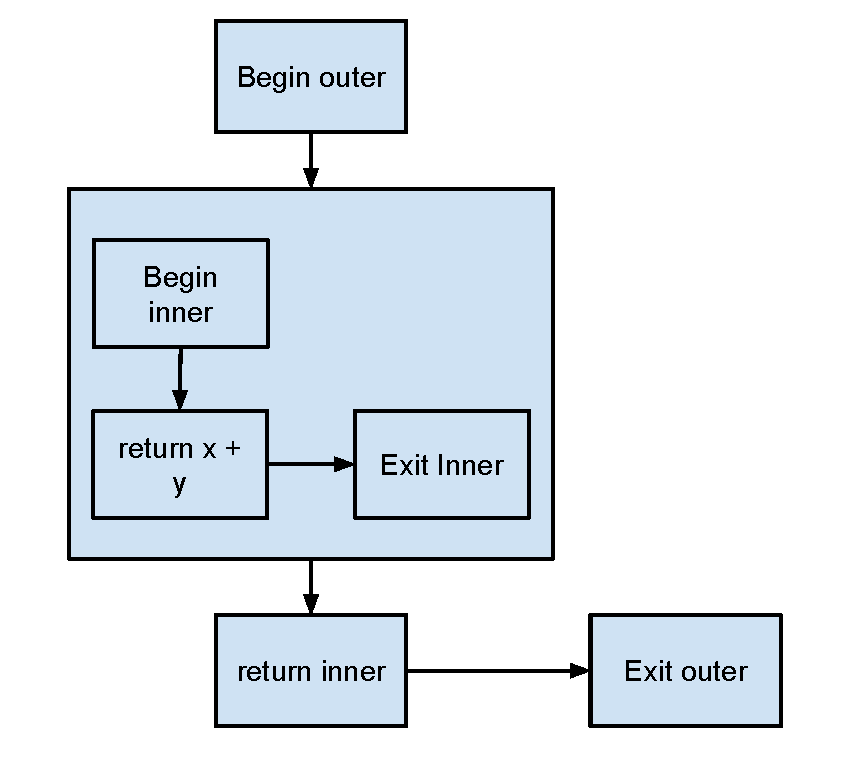
\includegraphics[scale=0.7]{images/dynamicFunctionCFG.pdf}
\caption{The control flow graph generated for the dynamic creation of a function. `Begin' and `Exit' blocks have been added for each function to increase clarity.}
\label{fig:dynamicFuncCFG}
\end{figure}


\newpage
\section{Evaluation}
\label{chap:evaluation}
Python can be used in many different kinds of projects. From single module scripts with no classes to larger projects across multiple modules and classes. In the interest of seeing how our tool performs on  all possible types of Python source code, we tested with a combination of these. \\
\indent In order to see how it runs on genuine scripts, samples have been taken from those posted in an online discussion~\cite{pythonScripts}. \\
\indent The larger projects have been taken from the beginning of the list of all open source Python3 projects on the Python package index, Pypi~\cite{python3Projects}.

	% Projects
	\begin{table}[bp]
	\centering
    \begin{tabular}{ | c | c | c | c | c | c |}
    \hline
     &  & \textbf{Num.} & \textbf{Num.}  & \textbf{Num.}  \\
    \textbf{Project Name} & \textbf{LoC} & \textbf{Modules} & \textbf{Classes} & \textbf{Functions} \\ \hline
    birthday-script & 37 & 1 & 0 & 2 \\ \hline
    subtitle-downloader & 49 & 1 & 0 & 2 \\ \hline
    futen & 178 & 2 & 1 & 14 \\ \hline
    fluent-logger-pyramid & 244 & 4 & 4 & 18 \\ \hline
    numconv & 352 & 3 & 1 & 3 \\ \hline
    cchardet & 602 & 2 & 2 & 47  \\ \hline
    sshmap & 1102 & 6 & 3 & 33 \\ \hline
    Glances & 6801 & 41 & 50 & 300 \\ \hline
    urllib3 & 6907 & 35 & 72 & 343 \\ \hline
    Requests & 17048 & 70 & 115 & 620 \\ \hline
    \end{tabular}
    \caption{Information regarding the projects used to test the tool. Given in ascending order by the number of lines of code. \texttt{birthday-script} and \texttt{subtitle-downloader} are scripts~\cite{pythonScripts}. All others are from Pypi~\cite{python3Projects}.}
	\label{table:toolTests}
    \end{table}
    


\subsection{False Positives}
The number of false positives issued per project can be seen in Table~\ref{table:toolResults}. The errors issued were determined to be false positives by manual checking. The highest number of false positives returned by any of the projects tested on, other than \texttt{urrlib3} and \texttt{Requests}, was two. However each of these false positives was the result of a feature not yet supported. For example, the two false positives in \texttt{sshmap} involve calling a function and providing arguments using the argument name. \\
\indent In the case of \texttt{urrlib3} and \texttt{Requests} the false positives issued propagated throughout the codebase resulting in the high number reported. \\
\indent It can be seen that as the size of the projects grow, the more likely it is that features not currently supported are used. Due to this our tool is currently best suited for small projects.

\subsection{Accuracy}
The greatest sources of inaccuracy in our tool is the use of built-in modules and being unable to infer the contents of container types. We will discuss the practical implications of each separately.

    % Results
    	\begin{table}
	\centering
    \begin{tabular}{ | c | c | c | c | c | c |}
    \hline
    \textbf{Project Name} & \textbf{Our Runtime} & \textbf{Pylint Runtime} & \textbf{False Positives} \\ \hline
    birthday-script & 0.2475 & 0.2334 & 0 \\ \hline
    subtitle-downloader & 0.2444 & 0.6609 & 0 \\ \hline
    futen & 0.1827 & 0.8556 & 0 \\ \hline
    fluent-logger-pyramid & 0.1474 & 1.1554 & 0 \\ \hline
    numconv & 0.6218 & 0.6118 & 0 \\ \hline
    cchardet &  1.9117 & 1.0991 & 0  \\ \hline
    sshmap & 1.9816 & 1.9566 & 2 \\ \hline
    Glances & 14.1534  & 7.8523 & 2 \\ \hline
    urllib3 & 13.3731  & 12.6151 & 74 \\ \hline
    Requests & 23.9292  & 51.2973 & 119 \\ \hline
    \end{tabular}
    \caption{The results of the tests. Each project was run 10 times. The runtime given is the mean of the runtimes. Times are given in seconds.}
	\label{table:toolResults}
    \end{table}

\paragraph*{Contents of Containers}\mbox{}\\
Some variation of a container type is used in every sample of Python source code we have looked at. They are frequently iterated over in \texttt{for} loops. This done in the following way: \texttt{for item\_name in container\_name}. The \texttt{item} is then used in the body of the loop for some purpose. Since we are unable to infer the types contained in the object we are required to assign \texttt{any} to the item. The use of the item in the body of the \texttt{for} then causes the \texttt{any}s to propagate. Similarly, any functions calls on a container which refer to the contents, or any direct accesses of the contents, such as indexing, will return \texttt{any}.

\paragraph*{Built-in Modules}\mbox{}\\
Built-in Modules, such as \texttt{re} and \texttt{os} have been used in all of our sample projects. Since these are not supported their identifier is given \texttt{any} type. Any function call or variable access made on these imports will return \texttt{any}. Anything but light use of these modules would see the inaccuracy propagate throughout the code. \\

\indent To demonstrate both of these, consider the following function taken from \texttt{birthday-script}:
\begin{lstlisting}[mathescape]
    def commentall(wallposts):
      """Comments thank you on all posts"""
      for wallpost in wallposts:

        r = requests.get('https://graph.facebook.com/%s' %
                wallpost['actor_id'])
        url = 'https://graph.facebook.com/%s/comments' % wallpost['post_id']
        user = json.loads(r.text)
        message = 'Thanks %s :)' % user['first_name']
        payload = {'access_token': TOKEN, 'message': message}
        s = requests.post(url, data=payload)

        print("Wall post %s done" % wallpost['post_id'])
\end{lstlisting}
where \texttt{requests} and \texttt{json} are built-in modules which have been imported and \texttt{TOKEN} is module-wide global \texttt{string}. In line 4 the parameter \texttt{wallposts} is iterated over. Since we are unable to infer the contents of containers the identifier \texttt{wallpost} is assigned \texttt{any} type. This means we lose type checking opportunities on line 7, line 8 and line 14. Similarly, due to the fact we have resorted to assigning \texttt{requests} and \texttt{json} the type \texttt{any}, on line 7, line 9 and line 12 the return types of the function calls are type \texttt{any}. The result of this is that \texttt{any} has been propagated to three variables, \texttt{r}, \texttt{user} and \texttt{s}. \\
\indent Due to our tool's inability to infer contents of containers and built-in modules, 4 out of 8 (50\%) of the variables created in this function have been assigned \texttt{any} type. \\
\indent However, in functions which do not use these features, such as mathematic calculations, our tool is reasonably accurate. Consider the following small function taken from \texttt{numconv}:
\begin{lstlisting}[mathescape]
    def int2str(self, num):
      """Converts an integer into a string.

        :param num: A numeric value to be converted to another base as a
                    string.

        :rtype: string

        :raise TypeError: when *num* isn't an integer
        :raise ValueError: when *num* isn't positive
     """
     if int(num) != num:
       raise TypeError('number must be an integer')
     if num < 0:
       raise ValueError('number must be positive')
     radix, alphabet = self.radix, self.alphabet
     if radix in (8, 10, 16) and \
              alphabet[:radix].lower() == BASE85[:radix].lower():
        return ({8: '%o', 10: '%d', 16: '%x'}[radix] % num).upper()
     ret = ''
     while True:
       ret = alphabet[num % radix] + ret
       if num < radix:
         break
       num //= radix
    return ret
\end{lstlisting}
where \texttt{self.radix} and \texttt{self.alphabet} are class variables which have been inferred as \texttt{any} due to being assigned parameters in the class \texttt{\_\_init\_\_} function and \texttt{BASE85} is a module-wide global \texttt{string}. Since \texttt{self.radix} and \texttt{self.alphabet} are classified as \texttt{any} the local variables \texttt{radix} and \texttt{alphabet} receive the \texttt{any} type on line 16. However, despite this, our tool infers the correct return type of the function as the type set \texttt{\{sting\}} as stated by the author in the function documentation. On line 22 we have a binary operation \texttt{+} on the left-hand \texttt{any} type and the right-hand \texttt{string} type. However our tool determines that the only legal outcome of this operation is \texttt{string} \texttt{+} \texttt{string} and so sets the return type of the binary operation as \texttt{string} only.

\subsection{Runtime}
The runtime of our tool and of Pylint can be seen in Table~\ref{table:toolResults}. The runtime of our tool is in-line with the runtime of Pylint. \\
\indent It is interesting to note that our tool either matches or slightly out-performs Pylint on all projects. A noticeable exception to this is the project \texttt{cchardet}. The stand-out difference between \texttt{cchardet} and other projects is that \texttt{cchardet} has noticeably higher ratio of functions to LoC and modules. A possible reason for this slower performance is perhaps that more functions result in more CFGs and a higher number of basic blocks. This would show the weakness of our naive approach to $\phi$ function generation and may result in the sub-par performance shown on this project.

\subsection{Bug Checking Capabilities}
Our system is capable of finding errors regarding the following:
\begin{itemize}
	\item Whether an identifier can be used as a base class
	\item Whether a get attribute can be successful
	\item Whether an identifier can be called
	\item Whether the correct argument types are given to a function
	\item Whether two identifiers can be used in a binary operation successfully
	\item Whether a \texttt{continue} is in a \texttt{finally} block
	\item Whether a \texttt{continue} or a \texttt{break} is outside of a loop
	\item Whether an \texttt{\_\_init\_\_} function returns anything other than \texttt{none} type
	\item Whether an object used as an iterator implements the \texttt{\_\_iter\_\_} method
	\item Whether an object used as an index implements the \texttt{\_\_getitem\_\_} method
	\item Whether an object used with the \texttt{in} operator implements the \texttt{\_\_contains\_\_} method
\end{itemize}
At this time our tool is not accurate enough to currently be used as a full-blown bug checker due to the limitations described in Chapter~\ref{chap:limitations}. For small programs with a limited amount of imports and container type use the tool is capable of finding fairly deep type bugs. However in programs which depend on built-in modules and containers currently our tool is only capable of finding basic programming errors due to the propagation of \texttt{any} types. These basic errors include mis-typing variable names and using the wrong variable in a statement.

\newpage
\section{Conclusion}
Throughout this project we have looked at types in programming languages, type inference and how it can be performed, we looked at how we can use techniques such as control flow graphs and single static assignment to create our system and how we can solve potential issues in Chapter~\ref{chap:designAlg}. We described the structure of our work, the trade-offs of our decisions and went on to evaluate it in a number of ways. We benchmarked our system against an existing type checker, looked at its accuracy and what errors it is capable of checking. \\
\indent This project aims to infer bugs involving type errors in Python code without the burden of having to check to see which errors are false positives and which are genuine. Our solution achieves this for small projects by using a flow-sensitive approach for local variables, a flow-insensitive approach for global variables, an algorithm based on success typings for inferring function arguments and a cautious approach to exceptions. This is done statically and out-of-the-box, without troubling the users with the technicalities of annotations. \\
\indent However our achievements are just the beginning in what could be a very promising line of work. It appears our solution may be usefully used alongside a more aggressive and false-positive sensitive tool.

\subsection{Future work}
The majority of the future work available is improving upon the accuracy of our tool. This can be done in the following ways:

\subsubsection*{Supporting Built-in Modules}
In order to build a type checker which can infer types accurately enough to become a tool of real use, the built-in modules need to be supported. Some built-in module was used in all of the examples we evaluated our tool on. Typing the import as the \texttt{any} type causes great inaccuracy to propagate through our analysis. However dealing with these modules is not simple. One possible solution would be to run our tool on these modules and use the types we are able to infer. Unfortunately, this is not a realistic option since a large number of Python built-in modules, such as \texttt{os}, are largely written in \texttt{C} for the purposes of speed. Parsing the modules by hand is also not a realistic option due to the sheer number of modules and their size. We believe that the best way to support these would be utilise the work of others, such as mypy~\cite{mypy}. Similar to the manner we supported built-in functions, mypy has inferred the types of functions and global variables within a number of these modules. At the time of writing, mypy's documentation of the modules is not complete. For example, there is currently no support for the \texttt{datetime} module. But with the most frequently used modules largely covered, such as \texttt{re}, \texttt{os} and \texttt{math}, there is certainly enough information to act as a promising starting point.

\subsubsection*{Calculating the Side-Effects of Functions}
As we saw in the Evaluation section, one of the greatest weaknesses of our tool is its inability to keep track of the types in container types. Due to the fact that most containers are mutable types, the side-effects of functions needs to be tracked before solving this problem becomes plausible. Calculating the side-effects of functions will also open the gateway to inferring the possible states of objects at a given point in the source code. \\
\indent To do this we need to analyse a function to determine the following:
\begin{itemize}
	\item What changes it may make to the global variables within the class
	\item What changes it may make to the the parameters given
	\item What other functions it may call
\end{itemize}
For example, consider the following function:
\begin{lstlisting}[mathescape]
    def f(x):
      y = 5
      x.append(y)
      self.f[y] = 5.0
      g()
\end{lstlisting}
Line 2 has no side-effects and so we ignore it. Line 3 makes a change to the parameter \texttt{x} by adding a type \texttt{int} to the contents. Line 4 makes a change to the global variable \texttt{self.f} and adds the type \texttt{int} to the keys and the type \texttt{float} to the values. On line 5 the function \texttt{g} is called and so any side-effects that the function \texttt{g} causes, we say that \texttt{f} also causes. \\
\indent If the function \textit{may} make cause a side-effect, such as if the change is within a \texttt{if} block, then a conservative approach may need to be taken and assume that it always causes it.

\subsubsection*{Tracking the Types of Elements in a Container Type}
The main problem involved in tracking the types of elements in a container type is the fact they are mutable. This problem is resolved by calculating the side-effects of functions since we are able to infer what changes functions may make to the elements of the container. \\
\indent As well as functions, types can be added through indexing, such as \texttt{some\_list[i] = value}. The types of the elements can be updated by adding the type of the value to the types of the elements. In some cases this index assignment may overwrite an element, possibly removing a type from the contents. However which element is overwritten  and how many elements need to removed before a container no longer contains elements of that type, is difficult to statically predict. A similar problem arises when an element of a container is removed using the \texttt{del} keyword described in Chapter~\ref{chap:del}. For instance, consider the following trivial example:
\begin{lstlisting}[mathescape]
    from random import randomint
    l = ["Hi", 5, 5.0]
    del l[randint(0, 2)]
\end{lstlisting}
This example will delete a random element from a \texttt{list} type. Since random numbers are being generated, it is impossible to statically predict which element, and therefore type, will be removed. A similar problem arises when a dynamic number of elements is added, such as when looping over a file and adding elements found until the end of the file is reached. In this case we cannot determine how many elements need to removed before we can safely remove the type from the types of the elements. A solution to this problem is to never remove any type inferred from the elements in a container.

%\subsubsection*{varargs and kwargs}
%TODO

\subsubsection*{Improving Exceptions}
Currently our tool assumes that all statements within a \texttt{try} block can cause an exception. This is, of course, not true. As an extreme example, the statement \texttt{pass} in Python has no effect, yet currently our tool assumes it is capable of causing an exception. Improving upon this will result in a boost in, both, accuracy and speed. The increased accuracy will result from the values of variables only being sent to the \texttt{finally} or \texttt{except} block if they are statements which can cause an exception. The speed of the tool will increase due to the fact that the CFG and SSA are required to do less work and their will be less $\phi$ functions to evaluate in the type checker. \\
\indent It would be not be simple to improve upon this method. One solution may be to determine which statements are capable of causing \textit{which} particular exceptions. Currently if there is more than one \texttt{except} block we link all statements to all possible \texttt{except} blocks. However this is often not accurate. For example, consider the following code:
\begin{lstlisting}[mathescape]
    try:
      x / y
      z[0]
      a = b + c
    except ZeroDivisionError:
      # Do something
    except IndexError:
      # Do something
\end{lstlisting}
Knowing that \texttt{ZeroDivisionError} statements can only be caused by a division and that \texttt{IndexError} can only be caused by indexing into a variable, greatly improve the accuracy of the tool. We would know to only link the block at line 2 to the block at line 6, to link the block at line 3 to the block at line 8 and that line 4 can cause none of the exceptions listed. This can also be done with \texttt{ImportError}, \texttt{KeyError}, \texttt{OverflowError}, \texttt{StopIteration} and \texttt{FileNotFoundError} to name a few. However dealing with user-defined exceptions would still remain very difficult and a cautious approach will still need to be taken.

\subsubsection*{Increasing `Magic' Function Coverage}
Our tool covers a number of `magic' functions, however there are a number, such as \texttt{\_\_add\_\_} and \texttt{\_\_ge\_\_}, which are currently unsupported. Each `magic' function performs a unique function and so must be considered separately. For brevity we will not describe the possible implementation procedures for each one. However magic functions such as \texttt{\_\_add\_\_} or \texttt{\_\_sub\_\_} take a parameter representing the value of the right-hand side of a binary operation. The result of this is the object may not necessarily be used in conjunction with it's own class type. For example:
\begin{lstlisting}[mathescape]
    class C():
      def __init__(self):
        self.total = 0
        
      def __add__(self, other):
        return self.total + other
\end{lstlisting}
In this case the class \texttt{C} takes only an \texttt{int} or a \texttt{float} as its right-side parameter. This means an acceptable use case for an instance of \texttt{C}, \texttt{c}, is: \texttt{c + 1}. Therefore, upon detecting a class implementing a method such as \texttt{\_\_add\_\_}, the possible types of the parameters need to be inferred before adding the class type and the parameter to the list of legal combinations for their respective binary operators.

\subsubsection*{The isinstance Function}
Python provides a built-in function, \texttt{isinstance}, to determine whether a variable is a particular type at a given point in the program. For instance, \texttt{isinstance(x, int)} will return true if \texttt{x} is an \texttt{int} type and false otherwise. Most occurrences of the function, from our experience, are used in dictating control flow, which gives us an opportunity to refine the set of types we have inferred for the target variable. Consider the following block of code:
\begin{lstlisting}[mathescape]
    if isinstance(x, int):
      # Do something
    else:
      # Do something
\end{lstlisting}
If we are able to determine that \texttt{isinstance} is being used to manage control flow then we refine our types for \texttt{x} in the \texttt{then} and \texttt{else} branches. For the \texttt{then} branch we can, assuming \texttt{x} is a local variable, create a new naming of it (in the same vein as SSA naming) which contains only the type \texttt{int}. We do the opposite for the \texttt{else} branch, we carry over all types \texttt{x} contains before the \texttt{if} minus the type \texttt{int}. So, if \texttt{x} has been inferred to the type set \texttt{\{int, string\}} before the \texttt{if}, in the \texttt{then} branch \texttt{x} would have the type set \texttt{\{int\}} and in the \texttt{else} branch \texttt{x} would have the type set \texttt{\{string\}}. If \texttt{x} did not contain the type \texttt{int} before the \texttt{if} the process would be the same. We would not retreat through the program and update our types for occurrences of \texttt{x} to, in this case, include the \texttt{int} type since we have to consider that the type being compared with the variable may have been chosen in error. \\
\indent All other uses of the function can be exploited in similar ways, the list comprehension \texttt{[isinstance(x, int) for x in list\_name]} will result in a \texttt{list} containing only the \texttt{int} type. If the types contained in containers are being tracked then this information can be used to refine the types of the new \texttt{list} being generated.

\subsubsection*{Improving the Speed}
The primary method of reducing the runtime of the tool would be to calculate the dominance frontiers of the basic blocks in the CFG before applying SSA naming. This would reduce the number of redundant operations performed in the type checker. This should result in a significant speed-up on projects with large functions with a large number of control flow constructs. This is due to the fact these functions are likely to have a large number of local variables and blocks which results in redundant $\phi$ functions.

%Throughout this project we have looked at the background of cryptography, access control and how they can be brought together to create our hierarchy, we looked at how we can use these to create our system and how we can solve potential issues in the \textit{Design} section. From there we described the structure of our work and went on to evaluate it in a number of ways. We benchmarked our system against Dropbox, looked at how potential users found using our system and what markets our work may perform well in, before finally looking at how secure our system is.
%\newline \indent This project aims to increase the automation in file sharing with different groups of friends who require different access control constraints. Our solution achieves this by using cryptography. This is done without troubling the users with technicalities. A user need not know what a `key' is, or how to derive and use them to access files. Most actions are performed in the GUI by selecting desired files and clicking the button for the desired action.
%\newline \indent We wanted our solution to be quick enough to be usable. From the \textit{Benchmarking} section we found that our solution comes with an overhead, as to be expected. Fortunately the most time consuming parts of our solution, registration and log in, only need be performed rarely. The most common actions a user is likely to perform, uploading and downloading files, bear little overhead, meaning our solution is a realistic one when it comes to performance. A performance which was in-line with Dropbox's performance.
%\newline \indent We wanted our solution to be secure, that is not to introduce any unnecessary threats to user. From the \textit{Security analysis} section we found no clear security holes in our work. With any security threats likely coming from `traditional' attacks.
%\newline \indent However our solution does not come without constraints. It requires the user to order the people they wish to share their files with in a fairly strict hierarchy. The degree to which most people can adopt this into their lives is yet to be seen and thorough case studies, or a release, would have to be done before we can know for sure. From the \textit{User stories} section we can see that there may be some people this suits well, while others may find the lack of flexibility frustrating. The division of these two sets of people is likely to be in the environment in which they intend to use our solution. It appears that our solution may be very useful in a business environment but may struggle to make an impact on a user who intends to use it in a social environment. Due to this we can see that our work may have a place alongside other file sharing software, like general file sharers, such as Dropbox, and collaboration software, such as Google Drive. Our potential users are organisations which have an inherently hierarchical structure, who may well find our solution a more efficient option than applications such as YouSendIt and Box.





\newpage
\appendix

\newpage
\section{\\Binary Operations} \label{App:AppendixBinary}
% the \\ insures the section title is centered below the phrase: Appendix B

\begin{longtable}{ |c |c |c |c | }
	\hline
	\textbf{Operator} & \textbf{Left Type} & \textbf{Right Type} & \textbf{Result Type} \\ \hline
	\multirow{4}{*}{$+$} & Int & Int & Int \\
						 & Int & Float & Float \\
						 & Int & Bool & Int \\
	                     & Float & Float & Float \\
	                     & Float & Int & Float \\
	                     & Float & Bool & Float \\
	                     & Bytes & Bytes & Bytes \\
	                     & String & String & String \\
	                     & List & List & List \\ 
	                     & Bool & Bool & Int \\
	                     & Bool & Int & Int \\
	                     & Bool & Float & Float \\
	                     \hline
	\multirow{4}{*}{$-$} & Int & Int & Int \\
	                     & Int & Float & Float \\
	                     & Int & Bool & Int \\
	                     & Float & Float & Float \\
	                     & Float & Int & Float \\
	                     & Float & Bool & Float \\
	                     & String & String & String \\
	                     & Bytes & Bytes & Bytes \\
	                     & Bool & Bool & Int \\
	                     & Bool & Int & Int \\
	                     & Bool & Float & Float \\
	                     \hline
	\multirow{4}{*}{$*$} & Int & Int & Int \\
	                     & Int & Float & Float \\
	                     & Int & Bool & Int \\
	                     & Int & String & String \\
	                     & Int & List & List \\
	                     & Int & Tuple & Tuple \\
	                     & Float & Float & Float \\
	                     & Float & Int & Float \\
	                     & Float & Bool & Float \\
	                     & String & String & String \\
	                     & String & Int & String \\
	                     & String & Bool & String \\
	                     & List & Int & List \\ 
	                     & List & Bool & List \\ 
	                     & Tuple & Int & Tuple \\
	                     & Tuple & Bool & Tuple \\
	                     & Bool & Bool & Int \\
	                     & Bool & Int & Int \\
	                     & Bool & Float & Float \\
	                     & Bool & String & String \\
	                     & Bool & List & List \\
	                     & Bool & Tuple & Tuple \\
	                     \hline
	\multirow{4}{*}{$/$} & Int & Int & Int \\
	                     & Int & Float & Float \\
	                     & Int & Bool & Int \\
	                     & Float & Float & Float \\
	                     & Float & Int & Float \\ 
	                     & Float & Bool & Float \\ 
	                     & List & List & List \\ 
	                     & Bool & Bool & Int \\
	                     & Bool & Int & Int \\
	                     & Bool & Float & Float \\
	                     \hline
	\multirow{4}{*}{$\%$} & Int & Int & Int \\
	                     & Int & Float & Float \\
	                     & Int & Bool & Int \\
	                     & Float & Float & Float \\
	                     & Float & Int & Float \\
	                     & Float & Bool & Float \\
	                     & String & Any\_Type & String \\ 
	                     & Bool & Bool & Int \\
	                     & Bool & Int & Int \\
	                     & Bool & Float & Float \\   
	                     \hline 
	\multirow{4}{*}{$**$} & Int & Int & Int \\
	                     & Int & Float & Float \\
	                     & Int & Bool & Int \\
	                     & Float & Float & Float \\
	                     & Float & Int & Float \\
	                     & Float & Bool & Float \\
	                     & Bool & Bool & Int \\
	                     & Bool & Int & Int \\
	                     & Bool & Float & Float \\  
	                      \hline 
	\multirow{4}{*}{$\&$} & Int & Int & Int \\
	                     & Int & Float & Float \\
	                     & Int & Bool & Int \\
	                     & Float & Float & Float \\
	                     & Float & Int & Float \\
	                     & Float & Bool & Float \\
	                     & Bool & Bool & Int \\
	                     & Bool & Int & Int \\
	                     & Bool & Float & Float \\
	                      & Set & Set & Set \\     
	                      \hline 
	\multirow{4}{*}{$|$} & Int & Int & Int \\
	                     & Int & Float & Float \\
	                     & Int & Bool & Int \\
	                     & Float & Float & Float \\
	                     & Float & Int & Float \\
	                     & Float & Bool & Float \\
	                     & Bool & Bool & Int \\
	                     & Bool & Int & Int \\
	                     & Bool & Float & Float \\
	                     & Set & Set & Set \\   
	                     \hline 
	\multirow{4}{*}{$\wedge$} & Int & Int & Int \\
	                     & Int & Float & Float \\
	                     & Int & Bool & Int \\
	                     & Float & Float & Float \\
	                     & Float & Int & Float \\
	                     & Float & Bool & Float \\
	                     & Bool & Bool & Int \\
	                     & Bool & Int & Int \\
	                     & Bool & Float & Float \\
	                     & Set & Set & Set \\        
	                     \hline               
	\multirow{4}{*}{$\ll$} & Int & Int & Int \\
	                     & Int & Bool & Int \\
	                     & Bool & Bool & Int \\
	                     & Bool & Int & Int \\
	                     \hline 
	\multirow{4}{*}{$\gg$} & Int & Int & Int \\
	                     & Int & Bool & Int \\
	                     & Bool & Bool & Int \\
	                     & Bool & Int & Int \\
	                     \hline    

    \caption{The built-in types which can be used together with binary operators and which type they will return as a result.}
    \end{longtable}




\newpage
\bibliography{mybib}{}
\bibliographystyle{plain}

\end{document}


